\documentclass[12pt]{article}

% Language setting
\usepackage[english]{babel}

% Set page size and margins
\usepackage[letterpaper,top=2cm,bottom=2cm,left=3cm,right=3cm,marginparwidth=1.75cm]{geometry}

\usepackage{amsmath}
\usepackage{multirow}
\usepackage{rotating}
\usepackage{pdflscape} % For landscape pages
\usepackage{booktabs} % For professional-looking tables
\usepackage{adjustbox}
\usepackage[colorlinks=true, allcolors=blue]{hyperref}
\usepackage{sectsty} % For customizing section titles
\usepackage{xcolor}  % For color definitions
\usepackage{floatrow}
\usepackage{graphicx}
\usepackage{url}
\usepackage[hyphens]{url} % Allows breaking URLs at hyphens
\usepackage{hyperref}
\hypersetup{
    breaklinks=true,
    colorlinks=true,
    linkcolor=blue,
    filecolor=magenta,      
    urlcolor=cyan,
}
\sloppy

% Define Dark Blue color
\definecolor{DarkBlue}{rgb}{0, 0, 0.55}

% Set section title color to Dark Blue
\sectionfont{\color{DarkBlue}}

% Change the color of the document title to bold and Dark Blue
\title{\textbf{\textcolor{DarkBlue}{A Comparative Life-Cycle Assessment of Sustainable Aviation Fuel (SAF) Pathways}}}

\date{December 13, 2024} 
\author{
    Aline Abayo \\ 
    Ahmed AlAli \\ 
    Marissa Marsh LoVullo \\ 
    Mohammed Rayes \\ 
    Oluwadamilare Hussein Orekoya
}

\begin{document}
\maketitle

\begin{abstract}
The aviation industry faces significant decarbonization challenges due to its heavy dependence on fossil-derived jet fuel. Sustainable aviation fuel (SAF) is a key pathway for reducing greenhouse gas (GHG) emissions in aviation and accelerating progress towards zero-emission goals. This study evaluated the performance of the life-cycle GHG emission measured in grams of carbon dioxide equivalent per megajoule of SAF produced (gCO\textsubscript{2}e / MJ) and the energy return on investment (EROI), the ratio of energy output to energy input (MJ/MJ) of two SAF production pathways: Hydroprocessed Esters and Fatty Acids (HEFA) from used cooking oil and soybeans and Alcohol to Jet (ATJ) from corn. The ATJ scenarios modeled did not achieve a 50\% reduction in GHG emissions compared to conventional aviation fuel, while the HEFA scenarios achieved a 48\% to 83\% reduction in emissions. 
\end{abstract}

\subsubsection*{Keywords} Sustainable Aviation Fuel $|$ Life-Cycle Assessment $|$ Carbon Emissions $|$ Aviation Decarbonization
\clearpage
\section{Executive Summary}
The aviation industry faces significant challenges in mitigating its environmental impact, contributing approximately 2.5\% of global carbon dioxide emissions. This environmental burden has led the sector to explore innovative solutions for decarbonization, with Sustainable Aviation Fuel (SAF) emerging as a critical strategy. SAF has the potential to reduce greenhouse gas (GHG) emissions and support the transition of the aviation industry to net zero emissions by replacing conventional kerosene-based jet fuel. This study provides a comprehensive life-cycle assessment (LCA) of two technologically mature SAF pathways, Hydroprocessed Esters and Fatty Acids (HEFA) and Alcohol-to-Jet (ATJ), focusing on their environmental performance in the context of the United States.

The scope includes an examination of life-cycle GHG emissions and energy return on investment (EROI) for SAF production pathways compared to conventional jet fuel. The LCA covers stages such as feedstock cultivation, production processes, transportation, and combustion, while excluding emissions related to infrastructure development. HEFA production pathways use lipid-based feedstocks, such as used cooking oil (UCO) and soybean oil, while ATJ production relies on corn-based ethanol, benefiting from the existing ethanol production infrastructure. This analysis employs the Greenhouse gases, regulated emissions and energy use in transportation (GREET) model to ensure accuracy and consistency in assessing the environmental performance of these pathways.

The study found significant variation in GHG emissions among SAF pathways. The HEFA pathway using UCO demonstrates the lowest emissions, at 16.9 gCO\textsubscript{2}e/MJ, due to its reliance on waste feedstocks that avoid farming and land-use change. HEFA derived from soybean oil shows higher emissions, at 39.7 gCO\textsubscript{2}e/MJ, largely influenced by the indirect land-use change (ILUC) impacts of soybean cultivation. ATJ produced from corn-based ethanol exhibits the highest emissions, at 72.1 gCO\textsubscript{2}e/MJ, driven by the energy-intensive nature of corn farming and associated ILUC impacts.

Energy efficiency, expressed as energy return on investment (EROI), also varies significantly across the SAF pathways. HEFA using UCO achieves the highest EROI of 5.3 MJ/MJ, reflecting its efficient energy utilization and reliance on waste-based feedstocks. HEFA derived from soybean oil delivers a moderate EROI of 2.2 MJ/MJ due to lower energy requirements in feedstock cultivation compared to corn. ATJ production records the lowest EROI of 1.24 MJ/MJ, highlighting the high energy demands of corn farming and ethanol conversion processes.

Each SAF pathway presents distinct trade-offs. HEFA offers lower GHG emissions but is constrained by the limited availability of lipid-based feedstocks like UCO and soybean oil. In contrast, ATJ benefits from the extensive ethanol production infrastructure in the United States but results in higher emissions and lower energy efficiency, primarily due to its reliance on corn as a feedstock.

The findings underscore the critical role of feedstock selection in determining the environmental sustainability of SAF production. Waste-based feedstocks, such as UCO, emerge as the most sustainable option due to their negligible land-use change impacts and high energy efficiency. However, the dependency on specific feedstocks poses challenges for scaling SAF production to meet the growing demand in the aviation sector.

To address these challenges, policies should prioritize the use of waste-based feedstocks to promote circularity and sustainability. Investments in advanced SAF production technologies, such as Power-to-Liquid (PtL), are essential for achieving long-term decarbonization goals. Furthermore, strategic alignment of SAF production facilities near feedstock sources and airports can minimize transportation emissions, further improving the environmental performance of SAF.

Despite its promise, the scalability of SAF remains constrained by several factors. Limited availability of sustainable feedstocks restricts production capacity, while higher production costs compared to conventional jet fuel create economic barriers. Additionally, indirect impacts such as ILUC and competition with food supply must be carefully managed to ensure the long-term sustainability of SAF pathways.

In conclusion, Sustainable Aviation Fuel represents a critical pathway for decarbonizing aviation. While HEFA pathways offer immediate benefits, their scalability issues necessitate diversification into advanced technologies like PtL. To achieve net-zero aviation, coordinated policy support, technological advancement, and a focus on sustainable practices are imperative. This study provides a foundation for informed decision-making to balance environmental, economic, and operational goals in the aviation sector.

\section{Introduction}
Aviation plays a crucial role in modern global transportation, but its environmental footprint is substantial due to its heavy reliance on petroleum-derived kerosene. Countries worldwide have stressed the importance of capping the rise in global temperature to 1.5 degrees Celsius by 2100 through the Paris Agreement (Lau et al. 2024). The aviation industry contributes approximately 2.5\% of global carbon dioxide (CO\textsubscript{2}) emissions, making it a key area to reduce emissions to meet international climate goals (Lau et al. 2024). The aviation sector is challenging to decarbonize for many reasons, including high fuel density requirements, weight and safety constraints, and the relatively high cost required to enter the aviation fuel market (Merchant et al. 2022). Approaches to reaching net-zero emissions in the aviation industry are synthetic fuels from biomass, fuels derived from green hydrogen and atmospheric carbon dioxide, and the direct use of green liquid hydrogen (Dray et al. 2022). One technologically mature solution to aviation’s emissions problem, sustainable aviation fuel (SAF), has high energy density and net heat of combustion that resembles the weight and volume characteristics of conventional aviation fuel (Wang and Rijal 2024).  

The International Air Transportation Association (2024) projects moving away from conventional aviation fuel and re-capturing CO\textsubscript{2} emissions is critical to reaching net-zero emissions by 2050. SAF is derived from renewable resources, such as crops, agricultural waste, and used cooking oils. These feedstocks undergo chemical processes that make them chemically similar to traditional jet fuel, allowing them to be blended and used in existing aircraft without modifications. 
Two leading approaches to reducing carbon emissions associated with the aviation industry are mandating a carbon emission trading scheme and implementing the mandated use of SAF. Cui et al. (2023) systematically compared carbon emission trading schemes and the use of sustainable aviation fuel in Chain-foreign routes through projections of carbon dioxide and non-carbon dioxide emissions from 2023 to 2100. Their results show that SAF is more effective in controlling the pollutant emissions of aircraft than the European Union’s Carbon Emission Trading Scheme (EU ETS). However, the authors concluded that the most significant way to control emissions would be mandated SAF use and ETS policies to curb the effects of global climate change (Cui et al. 2023). These results highlight the importance of continuing research on the environmental impacts of SAF production as a favored solution in reaching net-zero emissions from aviation. 

In the United States, SAF development began with research and pilot projects by the U.S. Department of Energy and the Federal Aviation Administration in the early 2000s, focusing on alternative jet fuels. This culminated in ASTM International approving the first HEFA-based synthetic paraffinic kerosene in 2011, allowing up to a 50\% blend with conventional fuel. As of 2022, SAF accounted for less than 0.1\% of jet fuel consumed by the commercial aviation industry (U.S. Government Accountability Office 2023). Since then, SAF production has steadily increased, with a notable increase in domestic output from 5 million gallons in 2021 to 52 million gallons by mid-2024, and 11 SAF pathways have received ASTM International’s approval (Office of Energy Efficiency \& Renewable Energy 2024). 

Governments increasingly support the sector's decarbonization through fiscal support for SAF production and mandating SAF use. However, governments and international organizations are still developing specific decarbonization approaches to achieve net-zero aviation in 2050. The available literature on approaches to decarbonization heavily relies on SAF, which is not commercially available for the large-scale deployment required to meet net-zero goals. Additionally, the supply of necessary feedstocks for SAF production is insufficient for U.S. government goals for SAF production, given the current production technology (O’Malley et al. 2023). This research aims to support the development of comprehensive and informed policy recommendations to help organizations achieve their climate goals while ensuring continued economic growth and connectivity.


\section{Problem Statement}
Aviation’s dependency on fossil fuels makes it one of the most challenging sectors to decarbonize, with 2.5\% of global emissions attributed to this industry (Lau et al. 2024). While SAFs are a solution to reduce GHG emissions of aircraft, concerns about their life-cycle impact remain. This study addresses the need for a comparative evaluation of SAF pathways through a life-cycle assessment to understand their potential to mitigate aviation’s environmental impact.

\section{Questions to Answer}
\begin{itemize}
    \item How do ATJ, FT, and HEFA pathways compare with conventional jet fuel regarding life-cycle greenhouse gas emissions in grams of carbon dioxide equivalent per MJ of product and energy consumption?
    \item What are the trade-offs between different SAF production methods?
    \item What are the impacts of process type and location on SAF production in the United States on life-cycle greenhouse gas emissions?
    \item What are the critical environmental and economic challenges in scaling SAF production?
    \item Is there enough feedstock in the U.S. to produce SAF to supply the aviation industry?
\end{itemize}

\section{Background}

Recent literature has evaluated potential pathways to achieve decarbonization in the aviation industry. SAF is commonly viewed as one of the strategies to reach net-zero emissions as demand for aviation is expected to grow. 

Sacchi et al. (2023) quantified the efforts needed to mitigate the contribution of the European aviation fleet to global warming through a mixture of approaches. The study found that if aviation growth is sustained, fully mitigating the climate impacts caused by the European aviation sector will simultaneously require extensive Carbon Dioxide Removal (CDR), SAF, and other physical and market-based interventions that require significant energy, natural, and financial resources. In addition, the study suggests reducing air traffic demand is a good short- to mid-term solution while dually investing in the development of SAF and CDR (Sacchi et al. 2023).


In addition, Borgero et al. (2023) modeled the pathway to net-zero emissions. The researchers concluded that decarbonizing aviation will require large quantities of SAFs. The results suggested that an exponential growth of ethanol and biodiesel industries would be required to produce the 19.8 Exajoules of SAF necessary to achieve net-zero carbon emissions under business-as-usual (BAU) conditions in demand and energy intensity. Furthermore, the study underscored the uncertainty in the effects of aviation’s non-CO2 radiative forcing. Achieving a net-zero emissions sector would also rely on CDR ranging from 0.2 to 3.4 gigatonnes of CO\textsubscript{2}. They noted that if market-based mechanisms are less expensive than SAFs, airlines may seek to offset rather than reduce their combustion emissions; this argument emphasized the need to consider the cost-effectiveness of SAF production. 

Due to their identical chemical properties to kerosene, SAF is a “drop-in” fuel and a near-term solution for reducing aviation emissions. Pathways for SAF need to be approved by ASTM International to be blended with conventional fossil kerosene and interchangeable with existing infrastructures and jet engines (International Aviation Trade Association, 2024). Therefore, existing aviation infrastructure can remain in place while new production and blending facilities are developed to increase fuel use. 

There are several production and conversion pathways to produce SAF and a wide variety of possible biofuel feedstocks. To date, the ASTM has certified eleven conversion pathways. Alcohol-to-jet (ATJ) and hydroprocessed esters and fatty acids (HEFA) pathways are among the most mature, well-researched and commercially viable production processes for sustainable aviation fuels (International Aviation Trade Association, 2024). Other pathways include the following methods: Fischer-Tropsch (FT), FT-based pathways containing aromatics feedstocks (FT-SKA), hydroprocessed fermented sugars (SIP), isobutanol and ethanol alcohol-to-jet (ATJ), catalytic hydrothermolysis jet (CHJ), hydrocarbons HEFA (HC-HEFA), co-hydroprocessing of FT hydrocarbons in a conventional petroleum refinery, and co-hydroprocessing of esters and fatty acids in a convention petroleum refinery (International Civil Air Organization 2022). Calderon et al. (2024) note that not one pathway will be able to meet all the SAF demand; instead, a composition of multiple pathways and feedstocks is necessary to meet the aviation industry’s projected demand. However, due to data availability constraints, we were unable to include analysis for all the pathways. 


The following sections expand on conventional aviation fuels as well as the two most technologically mature SAF production pathways: hydroprocessed esters and fatty acids (HEFA) from used cooking oil and soybeans and alcohol-to-jet (ATJ) from corn. The background information from existing literature and the life-cycle of each fuel type is discussed.


\subsection{Conventional Aviation Fuel }

\begin{figure}[H]
\centering
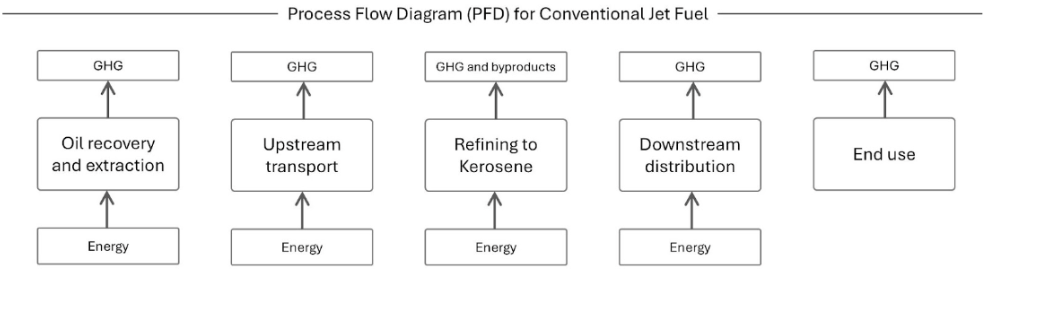
\includegraphics[width=0.8\textwidth]{Figures/Fig 1.png} % Replace 'fig10.png' with the path to your image file
\caption{A schematic overview of the conventional jet fuel supply chain and process flow diagram (PFD) used in this study}
\label{fig:figure 1}
\end{figure}

In the United States, the well-to-wake (WTW) life-cycle of jet fuel (kerosene) used in the aviation industry is produced through several key stages illustrated in Figure 1: extraction, refining, transportation, storage, distribution, and combustion (end use). Each stage consumes energy and contributes to greenhouse gas (GHG) emissions. These emissions are presented in units of CO\textsubscript{2}e, which accounts for CO\textsubscript{2} and other gas emissions expressed at the 100-year global warming potential from energy consumption throughout the life-cycle. This report will provide a detailed breakdown of emissions for each stage of the kerosene WTW life-cycle, as per studies by Jing et al. (2022) and Cooney et al. (2017), which was used for comparison. Table 1 shows data comparison, where each stage is explained in the following paragraphs.


\begin{table}[h!]
\centering
\label{tab:lca_emissions_comparison}
\begin{tabular}{|c|c|c|}
\hline
\textbf{LCA Stage (gCO\textsubscript{2}e/MJ)} & \textbf{Jing et al. 2022} & \textbf{Cooney et al. 2017 } \\
\hline
Drilling and Extraction & 9.6 & 10.6 \\
Refining and Distillation & 4.5 & 2.4 \\
Transportation of Kerosene & 0.8 & 0.7 \\
Storage of Kerosene & 0.1 & 0 \\
Distribution of Kerosene & 0.8 & 0.8 \\
Combustion & 73.8 & 73.7 \\
\hline
\textbf{Total} & \textbf{89.6} & \textbf{88.2} \\
\hline
\end{tabular}
\caption{The total well-to-wake emissions for kerosene in the U.S. are 89.6 and 88.2  gCO\textsubscript{2}e/MJ adapted from Jing et al. 2022 and Cooney et al. 2017, respectively.}
\label{tab:kerosene_emissions}
\end{table}


Extraction is among the most energy-intensive stages in the life-cycle, contributing 9.6 gCO\textsubscript{2}e/MJ in the U.S. (Jing et al., 2022). This reflects emissions from energy consumption and supplementary activities such as drilling and recovery processes, which are more energy-intensive due to the heavier crude oils typical of U.S. production. Cooney et al. (2017) extraction figure is slightly higher with 10.6 gCO\textsubscript{2}e/MJ, see table 1. The study adds granularity by categorizing U.S. petroleum production into Petroleum Administration for Defense Districts (PADDs). For instance, PADD 3 (Gulf Coast) dominates U.S. production and refining, while PADD 2 (Midwest) processes domestic and Canadian heavy crudes, resulting in higher extraction emissions compared to regions like PADD 4 (Rocky Mountain), where lighter crudes are more prevalent. These regional differences highlight the variability in lifecycle emissions within the U.S. However, the study averages all PADD regions to a U.S. average.

Refining in the U.S. results roughly in 4.5 gCO\textsubscript{2}e/MJ (Jing et al. 2022). Cooney et al. (2016) identifies that refining emissions vary significantly across PADDs with a US average of 2.4 gCO\textsubscript{2}e/MJ. While ICAO’s Carbon Offsetting and Reduction Scheme for International Aviation (CORSIA) model estimates refining to produce 1.7 gCO\textsubscript{2}e/MJ, this number is underestimated and biased since it was obtained from U.S. oil refineries (ICAO 2022). The refining stage involves fractional distillation, a process in which crude oil is heated and hydrocarbon products are separated, resulting in refined kerosene. U.S. refineries often use energy- and time-intensive deep conversion processes due to the need to process heavier crude oils. In contrast, countries like Saudi Arabia process lighter crude oil, which results in lower emissions during the refining stage. China and the European Union exhibit refining emissions similar to those of the U.S., mainly due to the complexity of the crude oil they process. (Jing et al. 2022).

Once refined, kerosene is transported to distribution centers via pipelines, trucks, and rail. The transportation stage in the U.S. adds 0.8 gCO\textsubscript{2}e/MJ to the life cycle emissions. Cooney et al. (2017) emphasizes the dominance of pipeline transport in PADDs 2 and 3, which reduces transportation emissions compared to PADD 4 and PADD 5 (West Coast), where rail and marine transport are more common. While, total US average is 0.7 gCO\textsubscript{2}e/MJ (Cooney, 2017). This reflects the energy used to move kerosene across large distances in the U.S., a vast country with dispersed consumption points. In comparison, Saudi Arabia, with its more centralized refining and distribution infrastructure that mainly relies on pipelines, experiences lower transportation emissions (Jing et al. 2022).

Kerosene is stored at various terminals and airports before use. The storage stage has relatively low emissions, contributing about 0.1 gCO\textsubscript{2}e/MJ (ICAO 2022). Emissions from storage are associated with maintaining the product at bulk plants using storage tanks (Jing et al. 2022). Since storage tanks are closed roof systems, emissions rarely escape. Fugitive emissions typically appear in the truck loading stage, where trucks are being refueled for distribution.

The distribution of kerosene from storage terminals to airports results in an additional 0.8 gCO\textsubscript{2}e/MJ of emissions. Similar to transportation, this stage is influenced by the U.S.'s geography, where kerosene must be transported over long distances to reach major airports. Regions with smaller geographic areas, more centralized refining, and heavy reliance on pipeline distribution show lower distribution emissions.

The final and most significant contributing stage of the kerosene life-cycle is its combustion in jet engines during air cruising. The combustion of kerosene emits 73.7 gCO\textsubscript{2}e/MJ, which is by far the largest contributor to the total life-cycle emissions (Cooney, 2017). This accounts for the majority of greenhouse gases released. This figure is consistent globally, as jet fuel combustion processes are similar across countries. The U.S. total well-to-wake emissions for kerosene stand at 90.8 gCO\textsubscript{2}e/MJ, slightly above the global average of 88.7 gCO\textsubscript{2}e/MJ (Jing et al. 2022).

The extraction and combustion stages primarily drive the life-cycle kerosene emissions in the U.S. The total emissions of U.S. kerosene at 89.6 gCO\textsubscript{2}e/MJ is slightly higher than the global average due to the heavier crude oils processed and the energy-intensive refining practices. PADD’s model presents the U.S. results as 88.2 gCO\textsubscript{2}e/MJ, which is slightly lower due to differences in averaged refining values (Cooney, 2017). Comparing these figures to other regions, Saudi Arabia demonstrates the lowest emissions at 81.1 gCO\textsubscript{2}e/MJ, mainly due to its more efficient extraction and refining processes. The EU and China present values similar to those of the U.S., at 89.1 gCO\textsubscript{2}e/MJ and 89.7 gCO\textsubscript{2}e/MJ, respectively. Reducing U.S. kerosene life-cycle emissions should focus on improving refinery efficiency and exploring alternatives to fossil-based jet fuels. The high emissions from aircraft fuel combustion highlight the need for fuel alternatives like SAF, improved engine efficiency, and operational measures such as optimized flight paths to reduce aviation's environmental impact (Jing et al. 2022).


\subsection{SAF Production Pathways}

\begin{figure}[H]
\centering
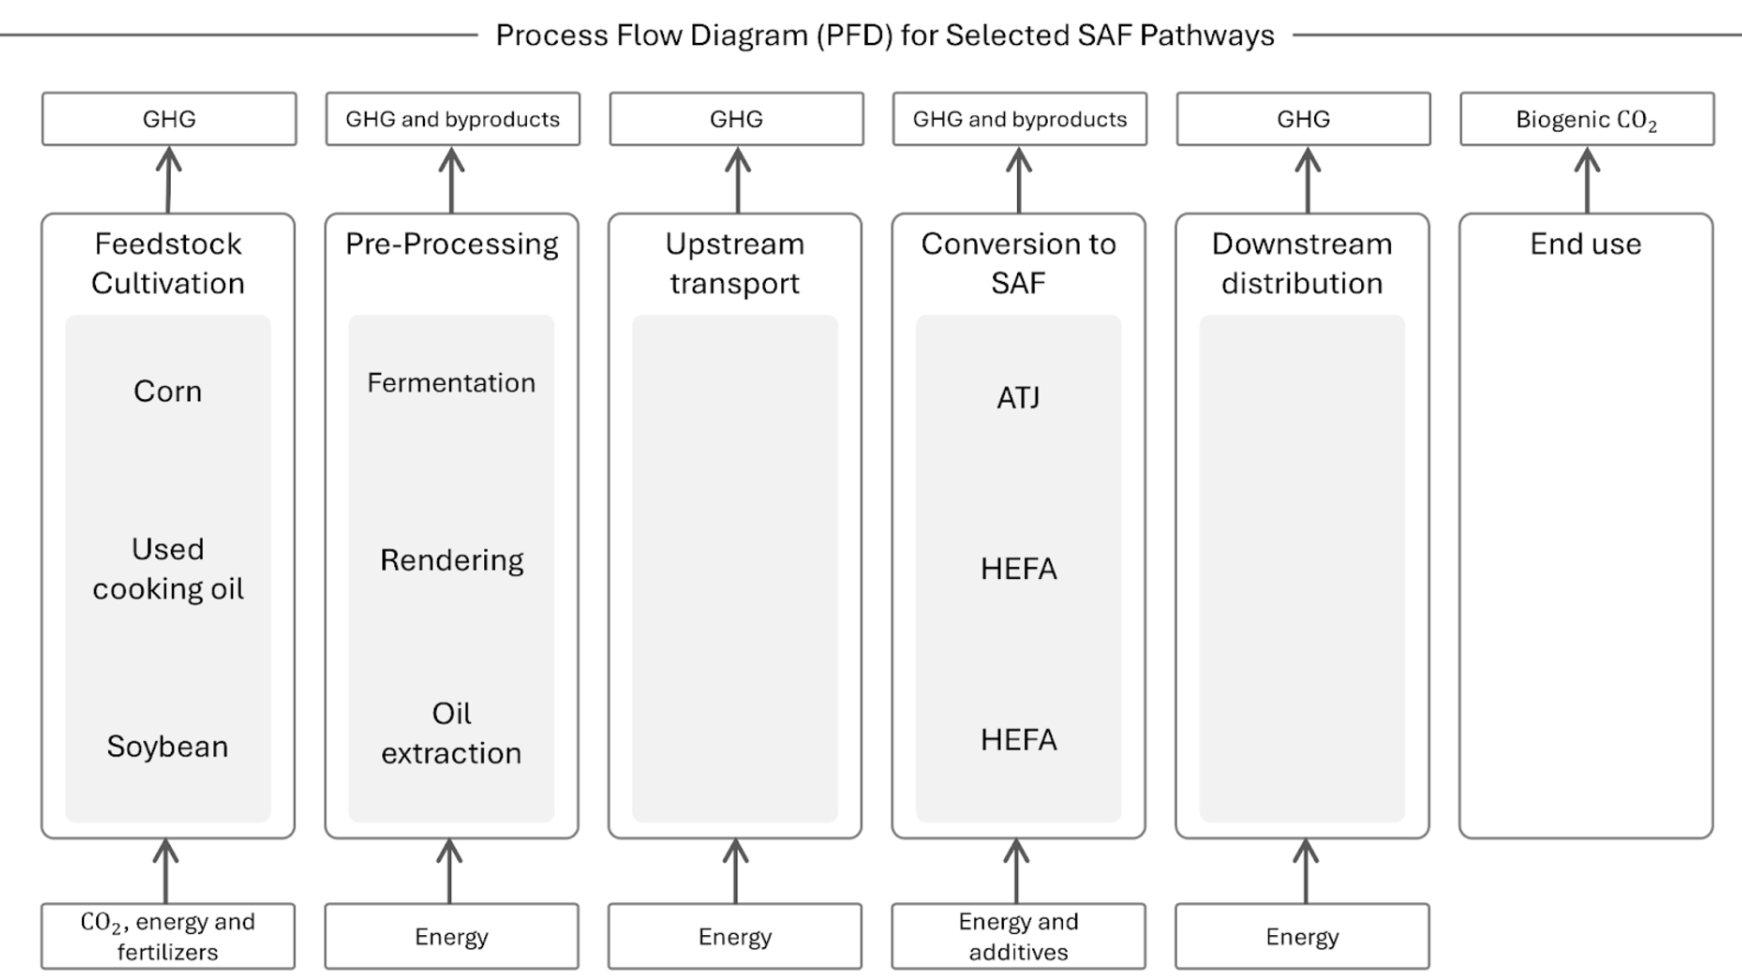
\includegraphics[width=0.8\textwidth]{Figures/Fig 2.png} % Replace 'fig10.png' with the path to your image file
\caption{A schematic overview of selected SAF pathways supply chain and the process flow diagram (PFD) used in this study}
\label{fig:figure 2}
\end{figure}

There are various ways to produce SAF from different production pathways and feedstocks. Stakeholders in the SAF industry state that the availability of SAF feedstocks is one of the top constraints of the industry’s growth (Calderon et al. 2024). Depending on geographic resource availability and demand, a combination of pathways and sustainable feedstocks may meet regional demand for SAF while minimizing the industry’s climate footprint.


\subsubsection{HEFA}

Hydroprocessed esters and fatty acid (HEFA) fuel is the market's most widely available and commercially viable SAF (Calderon et al. 2024). It has the highest energy conversion efficiency of the SAF pathways at 76\% (Lau et al. 2024). The life-cycle GHG emissions of HEFA SAF are approximately 27 to 55 gCO\textsubscript{2}e/MJ of SAF produced depending on the feedstock (de Jong et al. 2017). A low-carbon electricity grid and renewable hydrogen can further lower the fuel's carbon footprint. Mannion et al. (2024) compared embodied GHG emissions from current literature on HEFA feedstocks, which are included in the figure below. Unknown UCO refers to the uncertainty in the exact composition of waste cooking oil as a SAF feedstock in the figure below.

\begin{figure}[H]
\centering
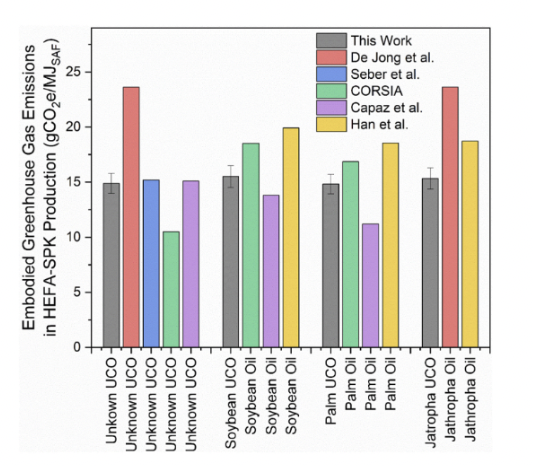
\includegraphics[width=0.8\textwidth]{Figures/Fig 3.png} % Replace 'fig10.png' with the path to your image file
\caption{Comparison of embodied emissions in HEFA feedstocks from existing literature reproduced from Mannion et al. 2024}
\label{figure 3}
\end{figure}

HEFA fuels are produced from various feedstocks. The following feedstocks are eligible for the 40B Provision of the Inflation Reduction Act’s sustainable aviation fuel credit: U.S. soybeans, U.S. and Canadian canola, used cooking oil, tallow, and distillers corn oil (Wang et. al 2024). The production of SAF by the HEFA pathway is limited by the availability of feedstocks, which considerably influences the fuel price due to the feedstocks' rising cost as demand from the biofuel industry grows (Lau et al. 2024). Algae oil is an emerging feedstock for HEFA SAF, but the Department of Energy projects that the feedstock may reach full-scale deployment around 2040 to 2050 (Calderon et al. 2024). 


\begin{figure}[H]
\centering
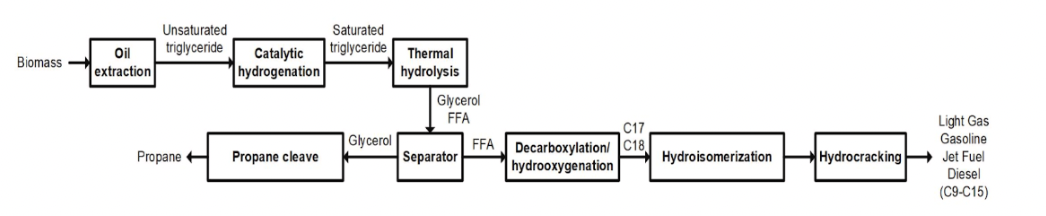
\includegraphics[width=0.8\textwidth]{Figures/Fig 4.png} % Replace 'fig10.png' with the path to your image file
\caption{HEFA production process reproduced from Lau et al. 2024}
\label{figure 4}
\end{figure}

The ASTM International approved hydroprocessed esters and fatty acids-synthetic paraffin kerosene as an aviation turbine fuel with a maximum percent blend rate of 50\% with conventional jet fuel. The HEFA process extracts oil from the biomass feedstock and transforms it through several chemical processes to become SAF. Feedstocks like wastes and animal fats are pretreated to remove impurities before refinement. Next, unsaturated fatty triglycerides are heated and hydrogenated with nickel, palladium, or platinum catalysts (Lau et al. 2024). The saturated triglycerides then go through thermal hydrolysis reactions to be broken down to glycerol that can produce propane and free fatty acids for further refinement to fuel (Lau et al. 2024). Next, the free fatty acids undergo decarboxylation or hydroxygenation at 300 to 600 degrees Celsius (Lau et al. 2024). A significant amount of hydrogen atoms are added as a catalyst to remove oxygen from the fats and oils, producing a pure hydrocarbon through the hydrodeoxygenation process (Wang et al. 2024). To lower the fuel’s freezing point, the pure hydrocarbons undergo hydroisomerization, coinciding with or after the hydrocracking process to produce SAF to meet ASTM properties suitable for flying at high altitudes (Lau et al. 2024). 

\begin{figure}[H]
\centering
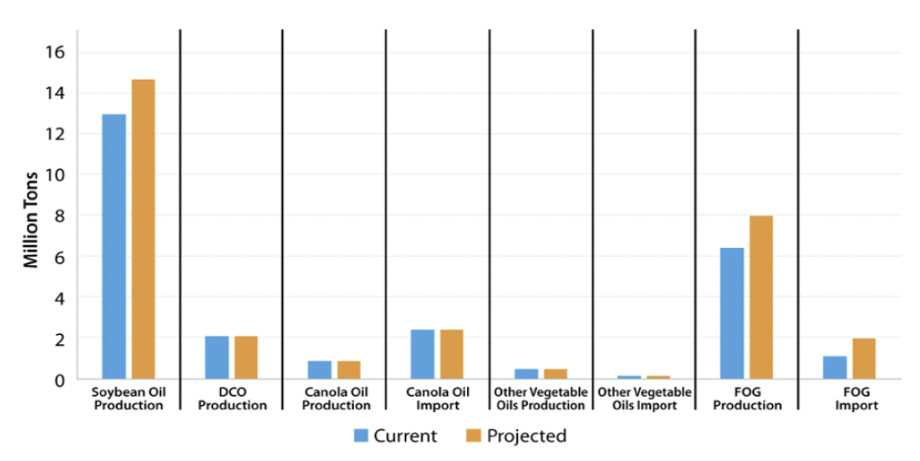
\includegraphics[width=0.8\textwidth]{Figures/Fig 5.png} % Replace 'fig10.png' with the path to your image file
\caption{Current and projected HEFA feedstock supply (2030-2032) reproduced from Calderon et al. 2024}
\label{figure 5}
\end{figure}


Used cooking oil (UCO), which also referred to as fats, oils, and greases (FOG) when combined with animal tallow and collected grease from wastewater facilities, is the second most abundant feedstock in the U.S. and has been evaluated for this comparative LCA for the HEFA pathway. The feedstock consists of UCO from commercial and industrial cooking operations unsuitable for human consumption (Calderon et al. 2024). Because UCO wastes are produced from various sources, a specific sample of the feedstock can be highly variable in terms of fatty acid content, thus resulting in differing energy conversion efficiencies (Mannion et al. 2024). The current production of UCO is estimated to be 1.4 million tons, geographically distributed throughout the country, with the highest production mirroring high population densities (Calderon et al. 2024).  Some biofuel producers prefer using inedible feedstocks like cooking oil and tallow over crops for food production, like Neste, which only uses wastes and residues for feedstocks (Calderon et al. 2024). Technological advancements and ground transportation electrification may result in more HEFA feedstock availability for SAF as facilities switch production from renewable diesel to SAF (Calderon et al. 2024). 

Soybean oil is a plentiful feedstock in the country. The U.S. is the second largest soybean oil producer in the world at 12.9 million tons, mostly from Illinois and Iowa (Calderon et al. 2024). However, soybean oil exports have decrease by 70\% over the past 10 years due to rising domestic demand of the biofuel industry (Calderon et al. 2024). Soybeans are transported to crushing plants, mostly located in the Midwest, before going to renewable fuel facilities which adds to the carbon intensity of HEFA SAF used in other geographic regions (Calderon et al. 2024). Hexane-based solvents, phosphoric acid, potassium hydroxide, sodium hydroxide, acid-activated bleaching earth, and other chemicals like antifoams are used for crushing and refining soybean oil (Calderon et al. 2024). Typical n-hexene emissions at crushing facilities exceed Environment Protection Agency air quality standards since it is a neurotoxin, posing a compliance difficulty for facilities using hexane to pretreat soybean oil for SAF production (Calderon et al. 2024). In the long term, soybean oil could be diverted from the road sector to aviation once hydrogen and battery-powered freight become widely utilized (O’Malley et al. 2023). 


\subsubsection{ATJ}

The alcohol-to-jet (ATJ) process allows for the sustainable production of kerosene from ethanol. Growing feedstocks for fuel production involves carbon sequestration, which offsets the CO\textsubscript{2} produced by combustion in later stages. ATJ typically converts alcohols, such as ethanol or butanol, into synthetic paraffinic kerosene, chemically identical to conventional jet fuel. The ATJ process is especially viable in regions like the United States, where corn grain is a primary feedstock for ethanol production. Corn accounts for 53.7\% of global ethanol production, making it a cornerstone in biofuel initiatives (Lau et al. 2024). The U.S. is the world’s largest producer of corn, offering a consistent and reliable domestic supply that is rarely affected by external uncertainties. Although more efficient processes such as HEFA and FT are also used in the SAF landscape, ATJ remains a popular choice due to its compatibility with the vast ethanol production infrastructure in the U.S. 
 
\begin{figure}[H]
\centering
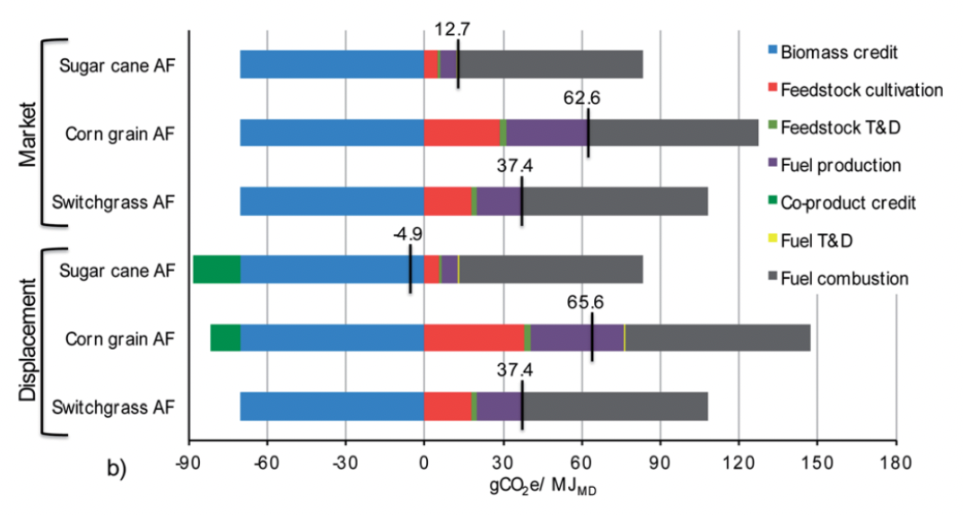
\includegraphics[width=0.8\textwidth]{Figures/Fig 6.png} % Replace 'fig10.png' with the path to your image file
\caption{Life-cycle GHG footprint breakdown reproduced from Staples et al. 2014}
\label{figure 6}
\end{figure}


 The life-cycle of ATJ fuel consists of the following stages: feedstock growth, feedstock cultivation, fuel production, and combustion. Growing the feedstock for ATJ is a carbon sequestration process that provides a “biomass credit” or negative CO\textsubscript{2} emissions. For corn, feedstock growth is valued at around -75 gCO2/MJ. Next are the most energy-intensive processes of cultivation and fuel production. Cultivation is the stage at which land is prepared for growing crops, including soil preparation, weed control, water use, and soil aeration. This stage is one of the most energy-intensive steps in “Corn-To-Jet” alongside fuel production. Fuel production includes biorefining corn into ethanol and upgrading ethanol, which is turned into jet fuel. There are four major steps in fuel production: dehydration, oligomerization, hydrogenation, and distillation. While hydrogenation is not an energy-intensive process, the hydrogen used in this step is largely produced via steam methane reforming (SMR), which is energy-intensive (International Energy Agency, 2019).  The cultivation process produces 37.4 gCO\textsubscript{2}/MJ, while the fuel production process produces around 40 g CO\textsubscript{2}/MJ. These values are summarized in Figure 6 above from Staples et al. (2014). Adding up the emissions from the life-cycle stages of corn-grain ethanol yields a value of 65.6 gCO\textsubscript{2}/MJ, the agreed default core LCA value for corn-grain ethanol (ICAO 2022).

 While corn grain dominates U.S. ethanol production, there is future potential for using cellulosic feedstocks such as corn stover, switchgrass, and agricultural residues to produce cellulosic ethanol. These feedstocks are derived from the non-edible parts of plants, such as the stalks, leaves, and husks, making them a more environmentally friendly option than food crops like corn grain. The appeal of cellulosic ethanol lies in its potential to reduce land-use competition between food and fuel, lower GHG emissions, and increase the overall sustainability of biofuel production. However, the economical scale production of cellulosic ethanol is not yet feasible and depends on many constantly changing factors, such as crop and energy prices. It also requires technological advancements and policy changes before it can be considered reliable (Aui et al. 2024). Figure 7 below shows the potential reduction of CO\textsubscript{2} emissions when comparing conventional jet fuel to SAF sourced from corn grain and corn stover feedstocks. Moving from corn grain to corn stover feedstocks offers 49.5 gCO\textsubscript{2}e/MJ reduction in emissions (Han et al. 2017). 

\begin{figure}[H]
\centering
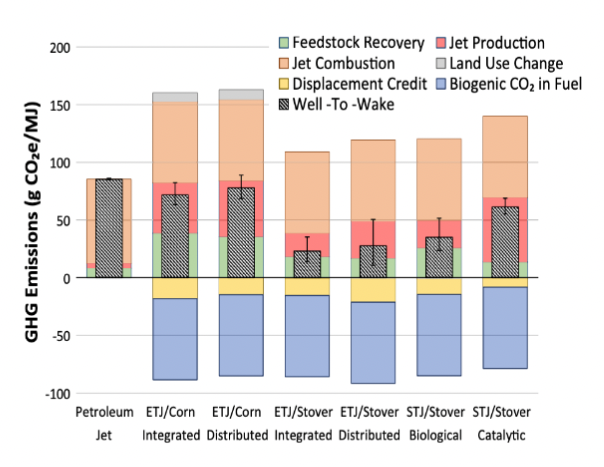
\includegraphics[width=0.8\textwidth]{Figures/Fig 7.png} % Replace 'fig10.png' with the path to your image file
\caption{WTWa GHG emissions of ETJ and STJ compared to petroleum jet reproduced from Han et al. 2017}
\label{fig:figure 7}
\end{figure}
 

\subsubsection{ Emerging SAF Pathways and Feedstocks}

While the HEFA pathway is the most technologically mature and commercially available feedstock, several pathways and feedstocks have the potential to drastically reduce GHG emissions while being sourced from waste and sustainable products. Fischer-Troupe and power-to-liquid (PtL) pathways are newer fuel pathway technologies. Algae is positioned as a unique feedstock since it does not compete for land and water due to its ability to be cultivated in low-quality environments like saline and wastewater (Langholtz et al. 2024). These pathways and feedstock will be discussed further in this section while not included in the scope of this report due to limited publicly available data. Fuel production includes biorefining corn into ethanol and upgrading ethanol, which is turned into jet fuel. There are four major steps in fuel production: dehydration, oligomerization, hydrogenation, and distillation. While hydrogenation is not an energy-intensive process, the hydrogen used in this step is largely produced via steam methane reforming (SMR), which is energy-intensive (International Energy Agency, 2019).  The cultivation process produces 37.4 gCO\textsubscript{2}/MJ, while the fuel production process produces around 40 g CO\textsubscript{2}/MJ. These values are summarized in Figure 6 above from Staples et al. (2014). Adding up the emissions from the life-cycle stages of corn-grain ethanol yields a value of 65.6 gCO\textsubscript{2}/MJ, the agreed default core LCA value for corn-grain ethanol (ICAO, 2022).

While corn grain dominates U.S. ethanol production, there is future potential for using cellulosic feedstocks such as corn stover, switchgrass, and agricultural residues to produce cellulosic ethanol. These feedstocks are derived from the non-edible parts of plants, such as the stalks, leaves, and husks, making them a more environmentally friendly option than food crops like corn grain. The appeal of cellulosic ethanol lies in its potential to reduce land-use change impacts.

Fischer-Tropsch (FT) is one of the most advanced methods to produce SAF, which is based on the synthesis of syngas from gasified biomass or waste and the conversion of syngas into long-chain hydrocarbons with the use of catalysts at high temperature and pressure. A key advantage of FT technology is its flexibility to utilize different types of feedstocks, including but not limited to non-food biomass and municipal waste, which makes it a flexible option for SAF production. The scalability of FT technology is attractive since it can leverage waste streams and renewable resources to produce SAF in regions with limited access to traditional bio-feedstocks. However, the process is currently capital and energy-intensive and requires advanced catalyst systems to optimize efficiency and product yield. Ongoing advancements in process efficiency and catalyst development are critical to enhancing the economic feasibility of this pathway, which holds substantial potential for meeting the decarbonization goals for the aviation industry (Shahabuddin et al. 2020).

Power-to-liquid (PtL) is an SAF production pathway that leverages renewable electricity and captured CO\textsubscript{2} to synthesize liquid hydrocarbons. This process involves three key stages: electrolysis to generate green hydrogen, CO\textsubscript{2} captured from the atmosphere, which also serves as the carbon source, and Fischer-Tropsch synthesis to convert hydrogen and CO\textsubscript{2} into liquid fuels. Current PtL values are placed at 21.43 gCO\textsubscript{2}eq/MJ (Rojas-Michaga et al. 2023).  PtL has the potential to achieve much lower lifecycle emissions if it uses 100\% excess renewable energy (International Renewable Energy Agency, 2021).

PtL fuels are particularly advantageous due to their scalability and independence from traditional biomass feedstocks, addressing land-use and resource constraints. They are classified as drop-in fuels, fully compatible with existing aviation infrastructure, and meet stringent safety and performance standards. However, the primary barriers to commercialization are the high energy demands and costs associated with the electrolysis and Fischer-Tropsch processes (Rojas-Michaga et al. 2023; IRENA 2021).  As the costs of renewable electricity and electrolyzers continue to decline, the PtL pathway is expected to play a critical role in meeting aviation's ambitious climate goals by providing a scalable and sustainable source of SAF.

Algae has emerged as a highly productive and efficient agricultural feedstock for SAF production, offering exceptional carbon efficiency. Open algae ponds can produce approximately 30 tons of biomass per acre, far surpassing crops like corn (7-8 tons) and soy (<0.4 tons of SAF precursors per acre) (Cox, 2022). With minimal land requirements, algae's scalability on non-arable land and wastewater resources enhances its potential for substantial greenhouse gas reduction, positioning it to produce billions of gallons of SAF annually and significantly contributing to decarbonization efforts.

Algae is the fastest-growing plant on earth and it can double its biomass in less than 24 hours, making it a highly efficient feedstock for SAF production (SAF Investor n.d.). Algae-based SAFs utilize sunlight, water, and nutrients to create fuel, following a "pond-to-plane" approach. Most SAFs are derived from biomass, such as crops like soy, corn, and microorganisms like yeasts or algae (Cox 2022). According to Cox 2022, scaling algae production to commercial levels could overcome one of the key challenges of SAF adoption—meeting the required production volumes to the required annual blending capacity—while achieving economic viability and reducing carbon emissions.


\textbf{\subsubsection{ Jet Fuel Demand}}

The United States’ average jet fuel consumption was roughly 52 million gallons per day for a total of  18.9 billion gallons in 2023 (U.S. Energy Information Agency 2024). To put this into perspective, global jet fuel demand this year has been 236 million gallons per day (Dareen and Khan 2024).  The SAF Grand Challenge adopted the goals of supplying at least 3 billion gallons of SAF per year by 2030 and sufficient SAF to meet 100\% of aviation fuel demand by 2050, which is projected to be around 35 billion gallons (U.S. Department of Energy Bioenergy Technologies Office 2022).  For context, SAF accounted for less than 0.1\% of jet fuel consumed by the commercial aviation industry in 2022 (U.S. Government Accountability Office 2023). 

\textbf{\subsubsection{ Price of SAF}}

SAF costs two to ten times more than conventional aviation fuel due to its higher production costs (Howe et al. 2024). Figure 9 details the variation in estimated price of SAF per gallon based on production facility designs and delivery cost to the airline. Additionally, these estimates are based on multiple feedstocks within each pathway including cellulosic products, waste products and virgin oils and crops. Offtake agreements between SAF producers and airlines have helped increase demand despite the cost premium of SAF as well as large technology companies and consulting firms seeking to reduce their Scope 3 emissions (Howe et al. 2024). While FT pathway SAF is projected to be low due to the low price of the waste feedstocks used, the technology is relatively immature to established pathways like HEFA and ATJ.
\begin{figure}[H]
\centering
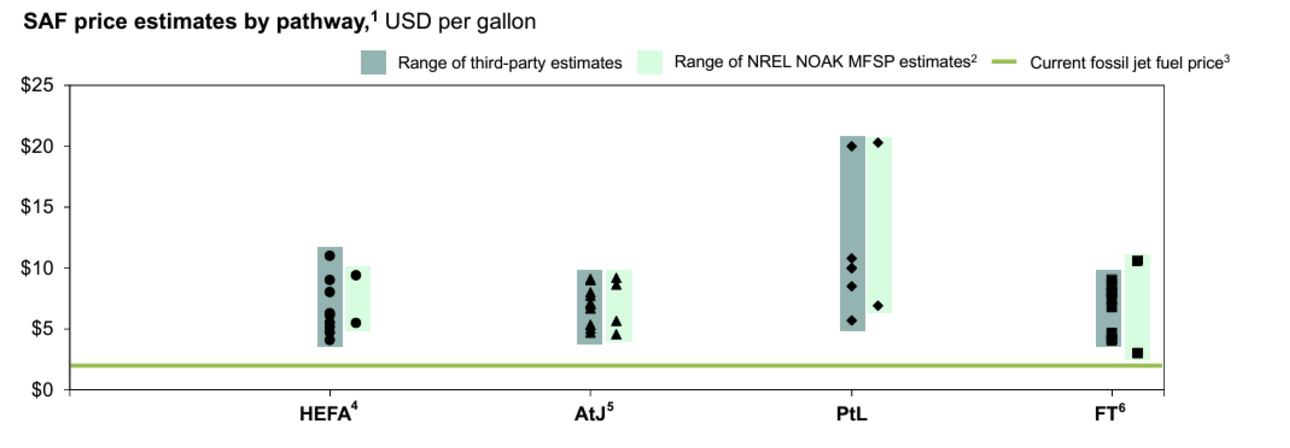
\includegraphics[width=0.8\textwidth]{Figures/price.png} % Replace 'fig10z.png' with the path to your image file
\caption{SAF price estimates by pathway reproduced from Howe et al. 2024}
\label{fig:price}
\end{figure}


\subsubsection{SAF Feedstock Availability}

The International Council on Clean Transportation estimated that the U.S. will have 12.2 billion gallons of SAF available from sustainably sourced domestic bio-feedstocks by 2050 (O’Malley et al. 2023). The breakdown of availability and SAF yield from the studied feedstocks are included in Figure 8. Corn grain ethanol and agricultural residues, such as stalks and husks of other farm products, have the highest theoretical yield of SAF. Competition from the road sector and consumer products limits the availability of ethanol and wastes, fats, and oils feedstocks to be converted to SAF (O’Malley et al. 2023). 

According to the CORSIA default Indirect Land Use Change values, soybean oil and corn grain ethanol did not meet the 50\% life-cycle GHG emission reductions as required by the 40B tax credit for the SAF Grand Challenge goals (O’Malley et al. 2023). However, under the Argonne National Laboratory model used to determine eligibility for the 40B tax credit, corn ethanol and soybean oil are considered sustainable due to differences calculating ILUC. This difference in accounting in LCA models will be discussed further in the Uncertainty section of this report.


\begin{figure}[H]
\centering
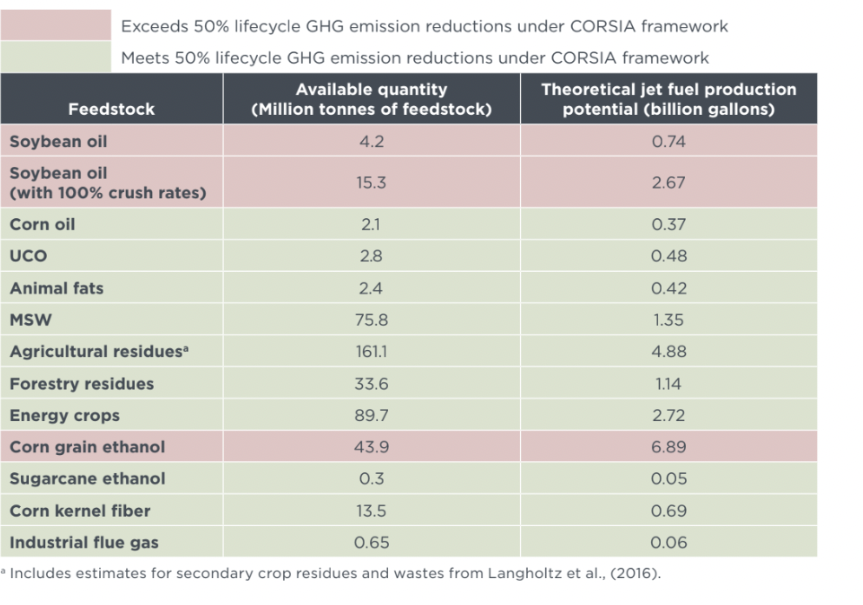
\includegraphics[width=0.8\textwidth]{Figures/Figure 10.png} % Replace 'fig10.png' with the path to your image file
\caption{Total theoretical U.S. SAF production potential by 2050 reproduced from O’Malley et al. 2023}
\label{fig:figure10}
\end{figure}

\subsubsection{U.S. Government SAF Initiatives }

The U.S. Department of Energy, Department of Transportation, and Department of Agriculture have launched the SAF Grand Challenge to accelerate the growth of SAF to decarbonize the aviation industry. The government has the goals of 3 billion gallons of domestic SAF production per year by 2030 and increasing to 35 billion gallons of production per year by 2050 to meet aviation’s domestic fuel demand, given that the fuel results in a minimum reduction of greenhouse gas emissions of 50\% compared to conventional fuel (Office of Energy Efficiency \& Renewable Energy 2024). The agencies have coordinated a voluntary reporting system to track progress toward the stated goals. Additionally, the above agencies and the Federal Aviation Administration have funded \$443 million in various research and development projects, including feedstock supply chain development, ASTM International investment, and SAF commercial deployment (Office of Energy Efficiency \& Renewable Energy 2024). 
This year’s SAF production is estimated to be 52 million gallons as of June 2024, predominantly from fat, oil, and grease feedstocks through the HEFA process (Office of Energy Efficiency \& Renewable Energy 2024). Domestic SAF production has risen from 5 million and 26 million gallons in 2021 and 2023, respectively (Office of Energy Efficiency \& Renewable Energy 2024). The Department of Energy estimates that SAF production last year reduced 154,000 to 216,000 metric tons of CO2e, based on an assumed 50\% to 70\% reduction from the HEFA production pathway (Office of Energy Efficiency \& Renewable Energy 2024). Based on the planned SAF projects, the coalition is optimistic that the domestic market will meet the 2030 production goal. 
A key driver in the increase of domestic SAF production is the federal SAF tax credit. The Inflation Reduction Act of 2022 established the Sustainable Aviation Fuel Credit. This tax credit applies to SAF sold or used during the calendar year 2024 that meets a minimum reduction of 50\% in life-cycle GHG emissions with higher credit rates available for further reductions (U.S. Department of Energy 2024). A SAF producer can claim \$1.25 for each gallon of eligible SAF (Internal Revenue Service 2024). The tax credit offers an additional \$0.01 for each percentage point greater than a 50\% reduction in GHG emissions (Internal Revenue Service 2024). Producers can also claim additional credit through further emissions reductions by employing established climate smart agriculture practices to cultivate corn and soybeans (Internal Revenue Service 2024). 

\section{Modeling Approach and Data}

\subsection{Approach}

This LCA study uses a cradle-to-grave assessment model, encompassing feedstock cultivation, production processes, transportation, and fuel combustion. The data for SAF pathways are sourced from the latest version of the greenhouse gasses, regulated emissions, and energy use in transportation (GREET) model using inputs and assumptions from peer-reviewed sources.  The 40B SAF tax credit version of the GREET model is used to conduct a comparative life-cycle assessment between conventional Jet A1 kerosene, ATJ SAF from corn feedstock, HEFA SAF from used cooking oil feedstock, and HEFA SAF from soybeans as feedstock. While the SAF pathways examined in this study are approved up to a  50\%  blend with conventional jet fuel, the model used in this study examined the life-cycle of SAF before it is blended with jet fuel. This decision allowed the results to evaluate if SAF was eligible for the 40B tax credit and aligned with federal climate initiatives. The functional unit for the project is gCO\textsubscript{2}e/MJ for GHG emissions and energy return on investment (EROI) in MJ/MJ.

\subsection{Model}

Domestic and international organizations have developed models to quantify SAF's life-cycle greenhouse gas emissions. These models have been employed to inform government policies, business investment, and tax incentives. The greenhouse gasses, regulated emissions, and energy use in transportation (GREET) model is widely used in the United States. The California GREET model has been adopted by the California Air Resources Board to model California-specific emission considerations. Internationally, the International Civil Aviation Organization has developed the CORSIA model to similarly model the life-cycle emissions of aviation. 


\subsubsection{Argonne National Laboratory’s GREET Model}

Argonne National Laboratory developed the greenhouse gasses, regulated emissions, and energy use in transportation (GREET) model to calculate the life-cycle of greenhouse gas emissions of various vehicle and fuel combinations. The model’s system boundary was expanded to include the well-to-wake analysis of aviation fuels and aircraft emissions for each unit of energy consumed by the aircraft or each unit of distance traveled (Elgowainy et al. 2012). The model includes HEFA from vegetable and algal oils (Elgowainy et al. 2012). Some of the latest updates to the GREET v1.3.0.14168 applicable to this project are life-cycle inventory of fertilizer and herbicide production, well-to-wheel life-cycle assessment of large agricultural tractor, and light-, medium-, and heavy-duty vehicles’ mass and characteristics (Wang et al. 2023).

\subsubsection{Argonne National Laboratory’s 40BSAF-GREET 2024 Model
}
The 40BSAF-GREET 2024 was released in April 2024 and last updated in October 2024 to examine SAF production pathways to calculate reductions in GHG emissions for eligibility for the 40B tax credit (U.S. Department of Energy 2024). The system boundary of the 40BSAF-GREET 2024 model includes all greenhouse emissions related to SAF production, from feedstock growth, feedstock processing, SAF production, fuel blending, and final use. The boundary also includes indirect emissions from production and transportation, as detailed below. 

\begin{figure}[H]
\centering
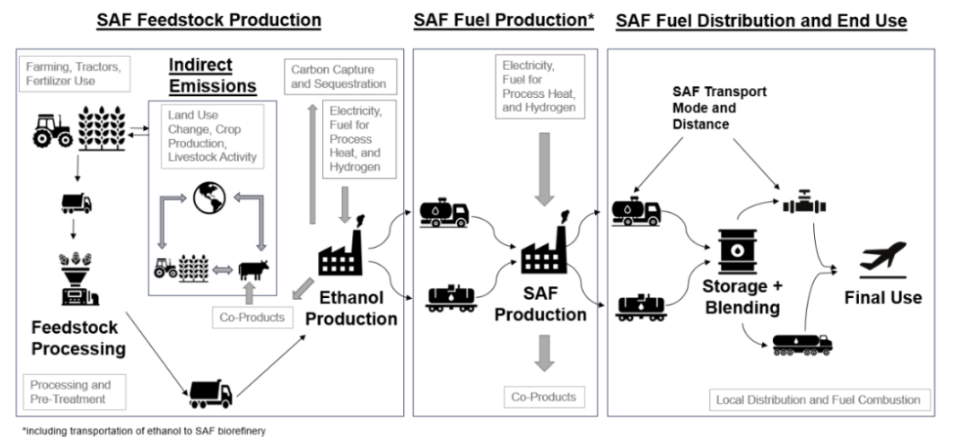
\includegraphics[width=0.8\textwidth]{Figures/Figure 11.png} % Replace 'fig10.png' with the path to your image file
\caption{SAF production GREET system boundary reproduced from U.S. Department of Energy 2024}
\label{fig:figure11}
\end{figure}

The functional unit of the model is 1 megaJoule (MJ) of fuel on a lower heating value IPCC basis. The calculated GHG emissions for the SAF are compared to a baseline of 89 gCO\textsubscript{2}e/MJ of conventional aviation fuel. The model assumes that one gallon of SAF equals the lower heating value of 126.37 MJ. Once the GHG emissions reduction is found, the model enables the user to claim the tax credit based on the gallons of SAF produced (U.S. Department of Energy 2024). The model uses the Intergovernmental Panel on Climate Change’s (IPCC) 100-year global warming potential of carbon dioxide (CO\textsubscript{2}), methane (CH4), and nitrous oxides (N2O) to determine the grams of CO\textsubscript{2}e produced per MJ of SAF produced (U.S. Department of Energy 2024). The model only calculates GHG emissions from the HEFA and ATJ, from ethanol feedstock, and production methods from seven distinct pathways produced in the United States but exempts Canadian canola and rapeseed and Brazilian sugarcane from the domestic production requirement (U.S. Department of Energy 2024). Additionally, there is no origin restriction on the tallow and used cooking oil feedstocks. However, the entire life-cycle of the feedstocks is still required, which may dissuade feedstocks with a high transportation impact (U.S. Department of Energy 2024). 

An important assumption of the GREET model is that CO\textsubscript{2} emissions from biogenic fuels are assumed to be offset entirely during the growth of biomass feedstock (U.S. Department of Energy 2024). Thus, the calculated value for the combustion stage only includes the non-CO\textsubscript{2} emissions from an aircraft, which is typically insignificant in magnitude relative to emissions in other stages. This assumption is similar to ICAO’s CORSIA model and is consistent with the IPCC Fifth Assessment Report (ICAO 2022). 

\subsection{Data}

Life-cycle assessments of sustainable aviation fuels often rely on data from the GREET model developed by the Argonne National Laboratory. One key feature of GREET is that it allows users to adjust various assumptions and parameters, such as land-use changes, feedstock types, energy inputs, and conversion efficiencies, which can significantly affect the final emission estimates. While this flexibility helps assess a wide range of biofuels and scenarios, it results in varying emissions data. On the other hand, the GREET model is a powerful tool for sensitivity analysis. 

This study originally sought to find input parameters to model ATJ and  HEFA pathways in the 40B GREET Model. However, sourcing the data from academic papers proved to be too difficult within the time constraints of this report. Instead, the sample LCA results for ATJ from corn ethanol and HEFA from used cooking oil and soybeans were selected. In the sensitivity analysis, the sample results were manipulated to estimate the emissions and energy return on investment of current SAF production in the United States through geographically specific grid compositions and transportation. 

\subsubsection{Sample LCA}

While developing the 40B SAF GREET model, Wang et al. found sample results from each of the SAF pathways of the model. The sample results are the direct and indirect greenhouse gas emissions from each pathway based on academic sources and industry surveys used to develop R\&D GREET. These results are based on the following assumptions: default parameters from R\&D GREET 2023, fossil natural gas for heat generations in ethanol and SAF production facilities, hydrogen generated from natural gas steam methane reforming in the SAF production, and the U.S. average electricity generation emission factor (Wang et al. 2024).  The direct life cycle GHG emissions are detailed in Table 2. below. The average emission factor was determined to be 520.89 kg CO\textsubscript{2}e/kWh from the average of the individual emission factors in the Energy Information Administration's 2023 Annual Energy Outlook. Transportation values listed in this table are calculated from R\&D Background data on feedstock sourcing, gathering, processing, and delivery to a SAF production facility (U.S. Department of Energy 2024). 

The sample LCA results were also used to determine the embodied energy calculations for the study’s second function unit of MJ/MJSAF. Assumptions about the process of upgrading ethanol to jet fuel were made based on data collected from ATJ producers and project developers in the U.S. and globally for the 40B-GREET model. These parameters were used in the embodied energy calculation and included in Table 3. Additionally, the default conversion rates in R\&D GREET 2023 were used in these calculations and are included in Table 4. 

\begin{table}[H]
\centering
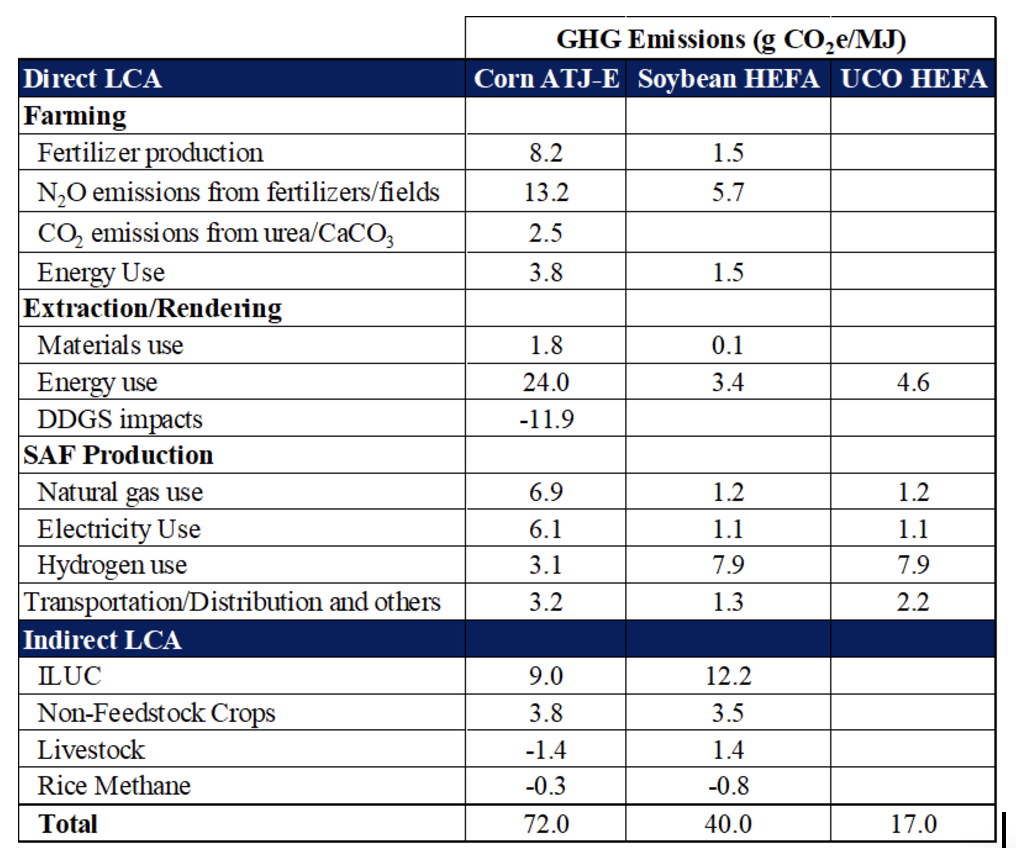
\includegraphics[width=0.8\textwidth]{Figures/tb2.png} % Replace 'fig10.png' with the path to your image file
\caption{Sample life-cycle emissions reproduced from Wang et al. 2024}
\label{tab:tb2}
\end{table}


\begin{table}[H]
\centering
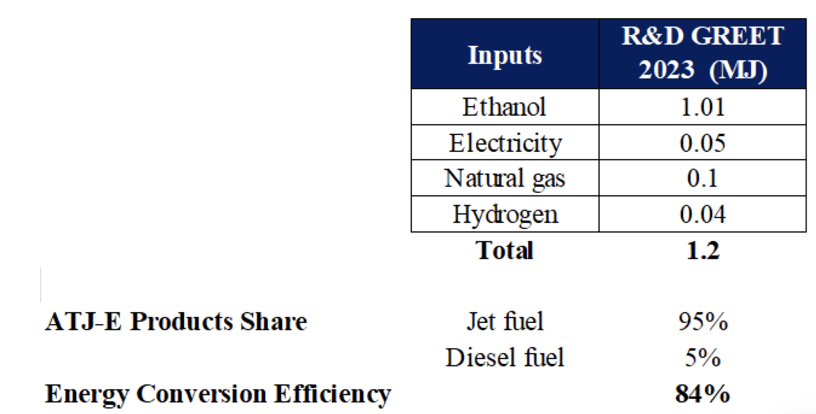
\includegraphics[width=0.8\textwidth]{Figures/tb3.png} % Replace 'fig10.png' with the path to your image file
\caption{ATJ corn ethanol default assumptions reproduced from Wang et al.}
\label{fig:tb3}
\end{table}

\begin{table}[H]
\centering
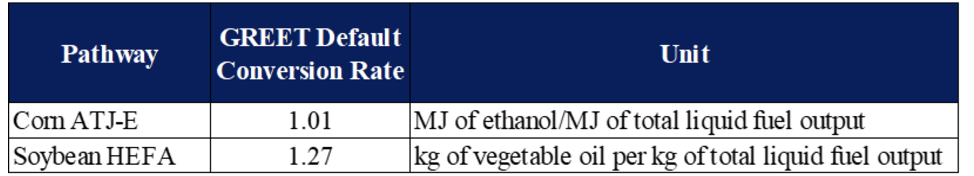
\includegraphics[width=0.8\textwidth]{Figures/tb4.png} % Replace 'fig10.png' with the path to your image file
\caption{R\&D GREET 2023 default conversion rates  reproduced from Wang et al.}
\label{fig:tb4}
\end{table}


\subsubsection{ Current SAF Production Modeling}

In the sensitivity analysis, the sample LCA results were manipulated to estimate current and projected SAF production facilities in the U.S. Data about the current state of the industry were primarily sourced from the National Renewable Energy Laboratory (NREL)  and the Department of Energy’s (DOE) reports. Figure 11. Below details current and projected SAF facilities. World Energy in Paramount, California and Montana Renewables in Great Falls, Montana are the largest HEFA SAF facilities in the nation. In a DOE webinar on November 24, 2024, Diamond Green Diesel was announced to have begun producing HEFA SAF instead of focusing on renewable diesel production. LanzaJet’s ATJ facility is currently operational but not producing SAF commercially at the time of this report. While there are many SAF production facilities anticipated to be operational before 2030, this report limited its scope to examining current and near-term SAF production since the 40B tax credit is set to expire in 2027 without renewal. 

\begin{figure}[H]
\centering
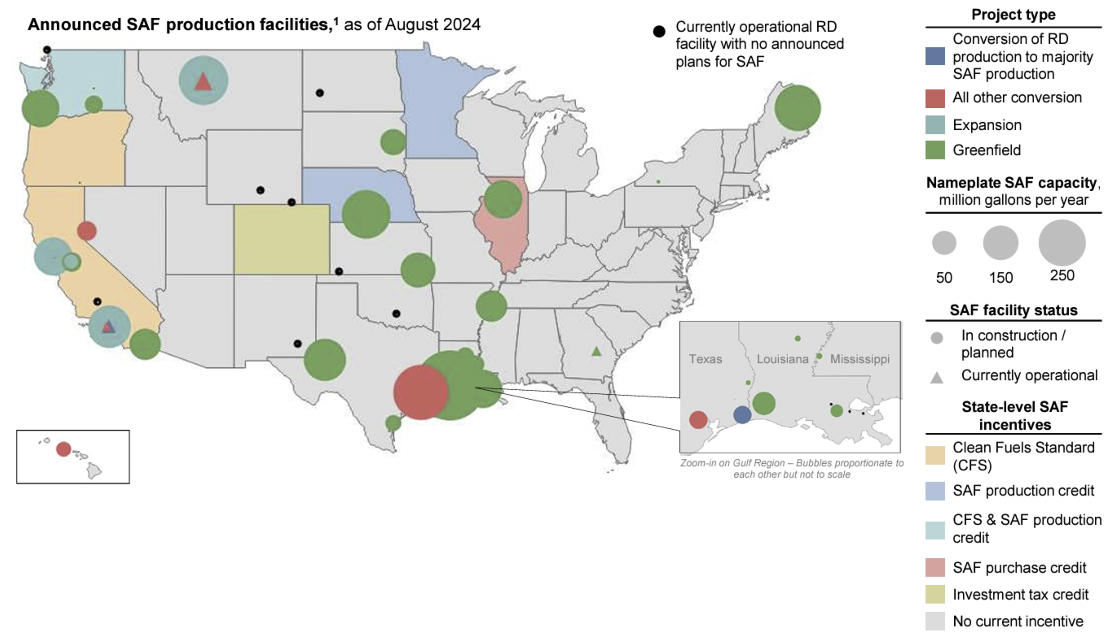
\includegraphics[width=0.8\textwidth]{Figures/Fig 12.png} % Replace 'fig10.png' with the path to your image file
\caption{R\&D GREET 2023 default conversion rates  reproduced from Wang et al.}
\label{fig:fig12}
\end{figure}

To model SAF use in the U.S., airports with current SAF supply were primarily examined. San Francisco International Airport (SFO), Los Angeles International Airport (LAX), O’Hare Airport (ORD), and Midway Airport currently are supplying commercial jets with blended SAF. Since O’Hare  and Midway airports are so close in proximity for the scale of the study, only O’Hare was modeled since Midway results would be so similar. Many U.S. airports have announced initiatives to supply SAF or partnerships with SAF producers in the future. A pipeline demonstration from Texas to LaGuardia Airport (LGA) was completed in 2022 as a demonstration of SAF use in existing fuel infrastructure (Bioenergy International 2022). To increase variability in the sensitivity analysis, LaGuardia was included in the scenario while it does not currently supply SAF. 

To estimate transportation emissions and energy, the supply chain of SAF production was researched using industry reports and company press releases. The 40B GREET model uses industry data on average used cooking oil collection, direct emissions at soybean crushing facilities, and corn delivery to ethanol facilities from background R\&D GREET models (U.S. Department of Energy 2024). Ethanol was assumed to be sourced from Iowa and Nebraska since those states are the two largest suppliers of ethanol in the country and have different grid compositions. Montana Renewables produces SAF and transports it to Crockett, CA to be blended with conventional jet fuel before the fuel is distributed to airports (Moriaty and McCormick 2024). World Energy on the other hand sends its SAF to be blended in a local refinery (Moriaty and McCormick 2024). A specific refinery could not be identified so a refinery in Wilmington, CA was selected to model typical emissions due to several refineries in the area in close proximity to the Port of Long Beach. LanzaJet announced that its SAF would be blended in Savannah, GA once the plant starts commercial production (Moriaty and McCormick 2024). According to NREL, SAF is likely being transported by trucks and rail. While SAF can use pipelines already in use for conventional jet fuel since its a drop-in fuel, pipeline deliveries have only been performed as demonstrations and announced for future use at production facilities once the industry is accustomed to accountability of SAF certifications in conjunction with conventional jet fuel. To overcome this uncertainty of the transportation mode of the SAF to blending facilities and later to airports, the study examined emissions from trucks as a worst case scenario model. 

To reflect local energy grid compositions, the ethanol and SAF production energy demand was extracted from the sample results using the average U.S. emission factor. An emission factor specific to the production facility was calculated using the composition of electricity generation sources multiplied by the emission factors from Horvath and Stokes (2011) and summarized in Table 5. To adjust the production GHG emissions to reflect the current ethanol and SAF production facilities location, the emission factor of city energy providers was multiplied with production energy demand to estimate production facility GHG emissions, assuming the production assumptions in the sample LCA reflected current conditions. The following local energy providers were used for this study: Nebraska Public Power District (2023), MidAmerican Energy Company (2024), Georgia Power (2024), NorthWestern Energy (2024), ComEd (Wattbuy 2024), and Entergy (2024). Production emissions could only be extracted for ethanol and SAF, so emission factors for ethanol production facilities and SAF facilities were found for this report. These calculated emissions factors are detailed in Appendix 1. Emissions associated with blending the neat SAF with conventional jet fuel were not within the scope of this study since the data could not be extracted from the R\&D 2023 Model. Additionally, the 40B Model does not account for the emissions from the 50\% blend since its purpose is to model neat SAF for the sake of tax credit eligibility. 
\begin{table}[H]
\centering
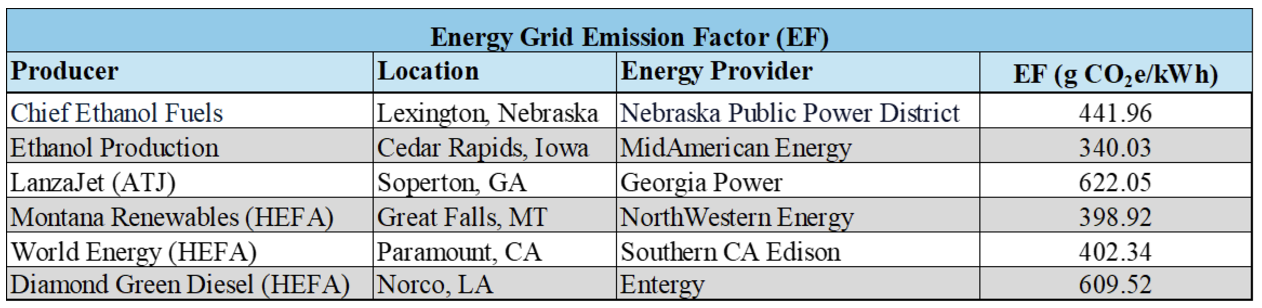
\includegraphics[width=0.8\textwidth]{Figures/factors.png} % Replace 'fig10.png' with the path to your image file
\caption{R\&D GREET 2023 default conversion rates  reproduced from Wang et al.}
\label{fig:factors}
\end{table}

\section{Results and Findings}
\subsubsection{GHG Emissions}

The results from the Wang et al. (2024) SAF LCA study indicated that the GHG emissions associated with SAF production and conventional jet fuel vary significantly depending on the feedstock pathway. These results, otherwise referred to as the sample LCA results, are included in Figure 12. The three combinations of SAF feedstocks and pathways explored in this study showed that ATJ-ethanol has the highest life cycle emissions of 72.1 gCO\textsubscript{2}e/MJ, largely due to farming, which accounts for 27.7 gCO\textsubscript{2}e/MJ and indirect land-use change ( 11.1 g CO\textsubscript{2}e/MJ). Major emission contributors are N\textsubscript{2}O from fertilizers/fields during farming (13.2 gCO\textsubscript{2}e/MJ) and energy use in production of ethanol (24.0 gCO\textsubscript{2}e/MJ).

HEFA-Soybean Oil produces moderate emissions of 39.7 gCO\textsubscript{2}e/MJ, with 16.2 gCO\textsubscript{2}e/MJ from ILUC and 10.1 gCO\textsubscript{2}e/MJ emission from SAF energy production. Its low emissions compared to ATJ-ethanol result from the absence of significant farming inputs and minimal processing requirements, as distillers corn oil is a by-product of ethanol production, avoiding additional agricultural burdens.

HEFA-UCO has the lowest GHG emissions of the three pathways at 16.9 gCO\textsubscript{2}e/MJ. It avoids farming and ILUC impacts. Its  emissions are primarily from SAF production (10.1 gCO\textsubscript{2}e/MJ) and transportation (2.2 gCO\textsubscript{2}e/MJ). These findings confirm the critical role of feedstock selection, highlighting that waste-based feedstocks like UCO have significant reduction in GHG emissions compared to crop-based alternatives.

\begin{figure}[H]
\centering
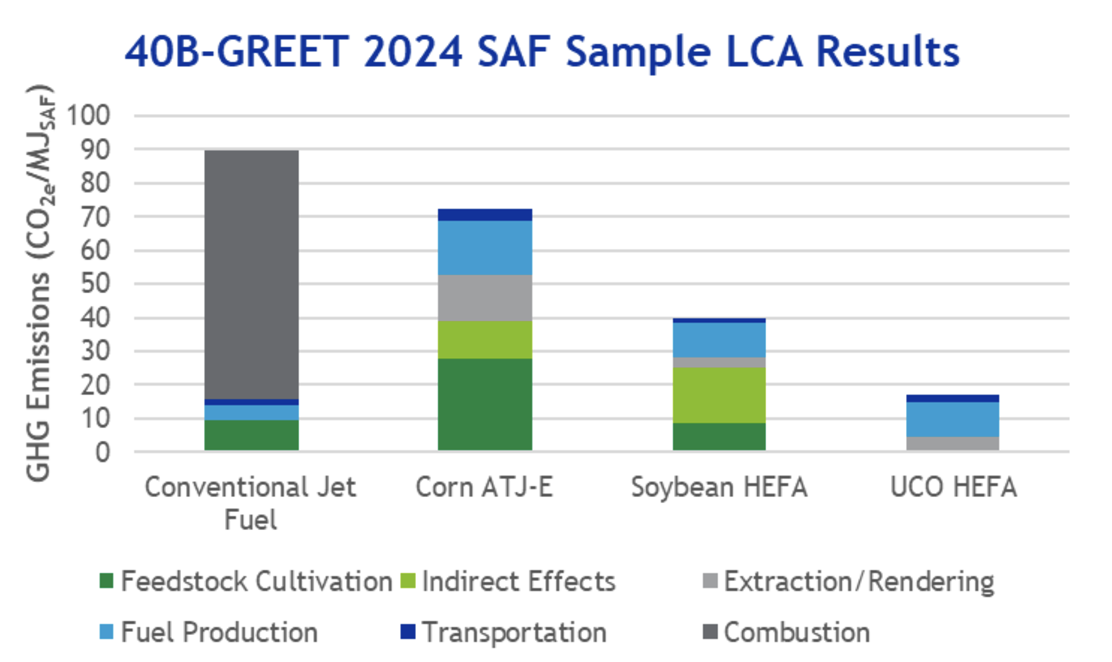
\includegraphics[width=0.8\textwidth]{Figures/samplelca.png} % Replace 'fig10.png' with the path to your image file
\caption{Sample LCA Results reproduced from Wang et al. 2024}
\label{fig:factors}
\end{figure}

\subsubsection{Energy Return on Investment}

The concept of Energy Return on Investment (EROI) provides a means to assess the "efficiency" of biofuel production processes by comparing the total emissions values of a certain pathway with conventional jet fuel. An EROI value greater than 1 indicates a net energy gain, with a value approaching 3 suggested as a minimum threshold for fuels within a sustainable society (Hall et al. 2009).

For SAF, EROI can be calculated on an LCA basis by comparing the emissions of conventional jet fuel to those of SAF (Trivedi et al. 2015). The EROI for corn ethanol, for instance, is calculated at 1.24, which is deemed inadequate for a sustainable fuel, though corn ethanol is an important transitional step especially considering the increasing supply of ethanol with the phasing of internal combustion engines and adoption of electric vehicles. Corn ethanol’s relatively low EROI is attributed to the high energy demands of corn farming and the subsequent biorefining and upgrading processes required to convert ethanol into jet fuel (Trivedi et al. 2015). The calculations of EROI for this study are included in Appendix 2.

The EROI of soybean oil is notably higher, at 2.2, nearly double that of corn. This increase is due to the less energy-intensive nature of soybean cultivation compared to corn. Furthermore, soybean oil can be directly converted into SAF using the HEFA process, which is more energy-efficient compared to the biorefining and upgrading processes required for corn ethanol. Soybean oil’s direct transformation into SAF bypasses the need for additional energy-intensive steps, reducing its overall energy footprint (Trivedi et al. 2015).

Finally, UCO achieves the highest EROI of all the feedstocks analyzed, with a value of 5.3. This high EROI results from the elimination of farming and ILUC impacts, coupled with the fact that UCO requires minimal processing before being converted into SAF. Rendering and conversion remain the most energy-intensive stages, but these are still more energy-efficient than the farming and biorefining processes associated with crop-based feedstocks (Hall et al. 2009).

Transportation energy costs for all processes were calculated to be positive, with tank trucks typically operating at a fuel efficiency of 6 mpg and a fuel capacity ranging from 3,000 to 11,000 gallons. For all scenarios examined in the sensitivity analysis, the truck’s fuel-carrying capacity exceeds the amount of fuel used, as the distances traveled were not large enough to generate negative values. 

\section{Sensitivity Analysis}

Varying the electricity grid and transportation distance to model the current U.S. SAF production revealed greater GHG emissions and therefore lower reductions than the sample LCA results from Wang et al. (2024). A summary of the modeled scenarios’ GHG reductions are detailed in Table 6 below. Table 7 lists the percent reduction of GHG emissions each scenario achieves compared to conventional jet fuel with the results color coded by if the SAF produced in the modeled scenario meets eligibility criteria for the 40B tax credit. Appendix 3 contains the complete results of the sensitivity analysis. Figure 13 details the SAF production phase breakdown between the best and worst Sensitivity Analysis scenarios, ATJ from Nebraska ethanol delivered to SFO and HEFA from UCO delivered to LAX, respectively, compared to the sample LCA values and conventional aviation fuel. 

The ATJ with corn ethanol and HEFA with soybeans generally failed to achieve similar results as the sample results. While HEFA with used cooking oil and soybeans modeled GHG emission results were 3\% greater than the sample LCA, ATJ with corn ethanol was 5\% greater than the sample LCA results. This increase is primarily due to the higher emission values from the assumed transportation of the feedstock to SAF production facilities which will be discussed further in Section 9.2. The HEFA pathway generally met eligibility criteria for the 40B tax credit by resulting in at least a 50\% reduction in GHG emissions with the exception of the scenario of LGA supplied with HEFA Soybean SAF from Montana Renewables. Similar to the sample LCA results, the modeled scenarios in the sensitivity analysis for LanzaJet production of ATJ SAF remained ineligible for the 40B credit. 

Overall, the HEFA-UCO pathway demonstrated the lowest emissions (16.9 gCO\textsubscript{2}e/MJ), largely due to its reliance on waste feedstocks that bypass farming and land-use change. This SAF production pathway and feedstock also achieved the highest EROI (5.3 MJ/MJ), reflecting efficient energy utilization.


\begin{table}[H]
\centering
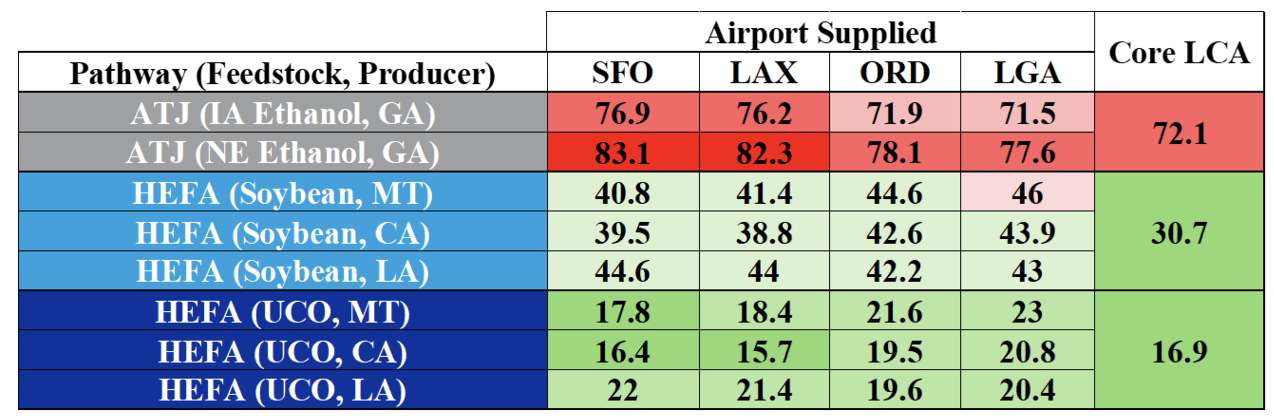
\includegraphics[width=0.8\textwidth]{Figures/num.png} % Replace 'fig10.png' with the path to your image file
\caption{Summary of sensitivity analysis results of greenhouse gas emissions of modeled SAF}
\label{table:num}
\end{table}

\begin{table}[H]
\centering
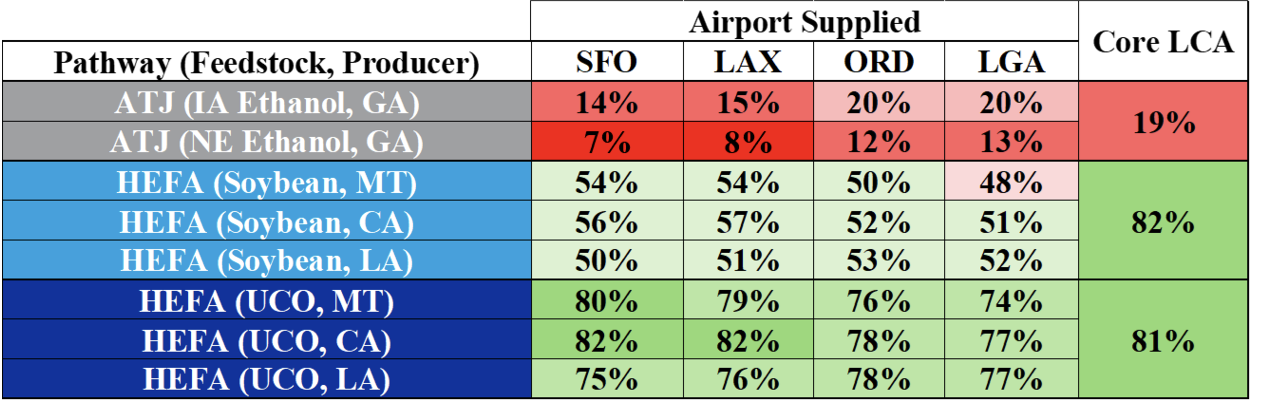
\includegraphics[width=0.8\textwidth]{Figures/perc.png} % Replace 'fig10.png' with the path to your image file
\caption{Summary of sensitivity analysis results for percent reduction of greenhouse gas emissions of modeled SAF scenarios}
\label{table:perc}
\end{table}

\begin{table}[H]
\centering
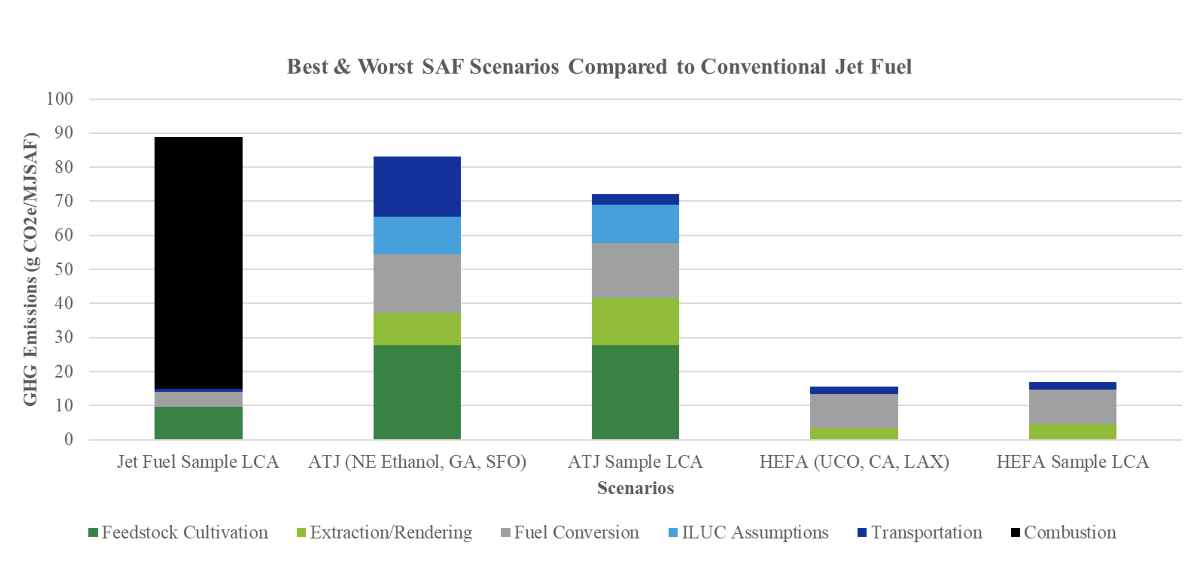
\includegraphics[width=0.8\textwidth]{Figures/bestworst.png} % Replace 'fig10.png' with the path to your image file
\caption{Best and worst modeled SAF scenarios compared to sample LCA results}
\label{table:perc}
\end{table}

\section{Uncertainty Assessment and Management}

\subsection{Data Quality}

Overall, high quality sources were found to model data in this study. A data quality pedigree matrix was developed as outlined in Junnila and Horvath (2005) and included in Appendix 4. The study’s data quality is summarized in Table 8. Representative data was sourced for key steps in SAF production. For example, data from 61 UCO rendering facilities was used to model the energy use and emissions associated with the rendering process (Wang et al. 2024). Corn farming data from the U.S. Department of Agriculture and industry surveys on ethanol production data formed the basis for Lee et al.’s (2021) study used in the 40B SAF GREET model. Argonne National Laboratory consulted multiple industry sources to obtain the best available corn to ethanol conversion data set in developing the R\&D GREET 2023 model (Wang et al. 2024). 

The 40B-SAF GREET model was based on Xu, et al. 2022 study on renewable diesel (RD) production, to model HEFA pathways of SAF production since there is limited publicly available data about the SAF production process. However, the technological process of SAF production and renewable diesel production is very similar as the HEFA conversion process typically generates both SAF and RD as products and HEFA conversion process data was collected from industry surveys (Wang et al. 2024). Both in the HEFA production pathway and renewable diesel production, a significant input of hydrogen is required to treat lipid’s triglycerides in the hydrodeoxygenation process (Wang et al. 2024). 

\begin{table}[H]
\centering
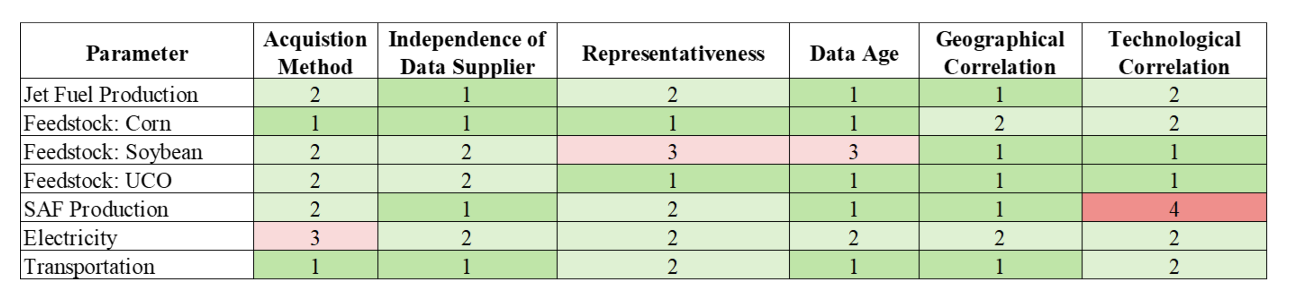
\includegraphics[width=0.8\textwidth]{Figures/dataqual.png} % Replace 'fig10.png' with the path to your image file
\caption{Summary Data Quality Analysis}
\label{table:perc}
\end{table}


\section{Interpretation and Discussion of Results}
ATJ and HEFA SAF pathways result in lower life-cycle GHG emissions than conventional jet fuel. However, the HEFA pathway, depending on the feedstock, results in less GHG emissions compared to ATJ. The following is a discussion of the implications of SAF production build-up related to this study’s results. 
In the sample and modeled LCA results in the sensitivity analysis, ATJ SAF failed to reach a 50\% reduction in GHG emissions. In this study, the lowest amount of GHG emissions ATJ SAF produced with corn ethanol resulted in 17.8 g CO\textsubscript{2}e/MJ or 20\% decrease in emissions. In the worst-case scenario modeled for ATJ, the SAF has merely 6.2 g CO\textsubscript{2}e/MJ savings or 7\% decrease. Even the CORSIA default value for ATJ SAF sourced from corn ethanol has GHG emissions of 65.7 g CO\textsubscript{2}e/MJ, which fails to meet the 50\% reduction compared to conventional aviation fuel (CORSIA 2022). 
Based on the results of this study, LanzaJet’s ATJ facility design likely varies from the base assumptions in the 40B-SAF GREET model. Given the current production price of SAF relative to conventional aviation fuel, the LanzaJet facility is likely designed to produce eligible SAF for the plant to be economically feasible. The facility may employ low-emission features like incorporating carbon capture and storage systems, heat integration, and adopting advanced catalysts to reduce costs and be potentially eligible for more tax credit. ATJ SAF and ethanol production facilities were assumed to be separate in the sample LCA results. GHG emissions and energy consumption could be reduced if the facilities were co-located to use the surplus heat and electricity from ethanol production to reduce natural gas and electricity requirements in the SAF process (Wang et al. 2024). 

\subsection{SAF Concerns}

Some trade-offs between different SAF pathways and feedstocks beyond differences in GHG emissions and energy demand are the sustainable feedstock supply and ILUC concerns. The HEFA pathway is the only technologically mature production method used commercially in the U.S. and is expected to produce 70\% of total SAF production in 2030 (Howe et al. 2024). While the 40B-SAF GREET methodology used in this study shows significant reductions in GHG emissions compared to conventional fuel, there is some disagreement among experts on the life-cycle emissions based on land use and economic levers. As the federal government has looked to increase SAF production, these areas have been extensively researched over the past 5 years. 

Not only are there concerns about purpose-grown fuel crops threatening food security, but also concerns that there is insufficient domestic sustainable biomass available to meet projected SAF demand by 2050 Grand Challenge goals.  The DOE’s 2023 Billion-Ton Report affirms that the U.S. can provide 1.7 times the biofuel feedstock demand for the SAF Grand Challenge 2050 goal, provided adequate markets can be established and that environmental safeguards are established to ensure sustainable outcomes (Langholtz et al. 2024). However, O’Malley et al. (2023) assert that insufficient sustainable biomass is available to meet the 2050 goal. Under CORSIA’s default ILUC values, soy and corn ethanol-derived SAF do not meet the 50\% reduction in GHG emissions required to be considered a sustainable feedstock, as discussed in the previous section. Furthermore, increased demand for soy for biofuel production has led to increased palm and soybean oil imports from Asia and South America which has a higher risk of causing deforestation to produce (Naverrete et al. 2024). Therefore, even though SAF production may be directly sourced from unsustainable feedstocks, the increased demand for these products may cause other sectors to use them. 

Even for SAF produced with waste feedstocks, there are scarcity concerns. U.S. producers have imported low-carbon and low-cost feedstocks, but studies have found that traceability and verification of these imported oils are challenging  (Howe et al. 2024). Virgin oils have been misleadingly labeled waste oil to satiate market demand (Naverrete et al. 2024). While imported used cooking oil is ineligible for the 40B tax credit, environmental guardrails for sourcing feedstocks, like feedstock verification, are essential to maintaining the integrity of life-cycle assessments of biofuel aimed to reduce GHG emissions. As the demand for waste products for RD decreases with projected battery and hydrogen-powered vehicles in the freight increases, these feedstocks can be redirected to aviation use. 

As mentioned in the Uncertainty Assessment, the quantified effects of ILUC have yet to be confidently known. Feedstocks like corn ethanol and soybeans may only meet GHG reduction targets depending on the calculated ILUC values and are primed to encourage further deforestation and the expansion of farmland (Naverrete et al. 2024).  The 40B credit encourages climate-smart agriculture practices, but the credit is more relaxed on crop based feedstocks in comparison to the European Union (EU). Under the ReFuel EU initiative, SAF cannot be produced from food crops like palm and soy due to sustainability criteria (Voegele 2023). 

For these reasons, power-to-liquid (PtL) technology using captured carbon dioxide is emerging as a favored SAF production pathway once it reaches technological maturity and economic feasibility (Howe et al. 2024). With a projected carbon intensity of 2.4 g CO\textsubscript{2}e/MJ and a domestic supply potential of over 15 billion gallons a year, PtL is a more promising sustainable pathway than the biofuel feedstocks examined in this study (Navarrete et al. 2024). The power-to-liquid feedstock is likely the future key long-term strategy to decarbonize aviation until hydrogen and battery-powered aircraft are technologically mature. 


\subsection{Scaling-up SAF}

SAF production facilities have been developed in states with clean fuel incentives, existing oil refinery facilities, and areas with high bio-fuel feedstock supply. Siting SAF production facilities with cleaner grid composition supports lower lifecycle GHG emissions, as reflected in the sensitivity analysis of the effects of electricity grid composition. Taking a lesson from the impact of feedstock shuffling from other states to California due to the high RD incentives of the Low Carbon Fuel Standard, state and federal policies to incentivize SAF use must be aligned to prevent additional GHG emissions from reaping higher economic rewards in different states (Naverrete et al. 2024). 

A concern regarding the SAF production build-up is social equity. Marginalized communities have historically carried the burden of the health consequences of living close to oil refineries and other high-polluting industrial sources. While locating SAF facilities near existing fuel refinery infrastructure or converting facilities to SAF production could decrease the fuel’s life-cycle carbon footprint, these actions will not improve the negative health impacts faced by people living in the surrounding area of the plant. Implementing emissions control technologies in SAF production facilities could reduce the negative health impacts on neighboring communities (Naverrete et al. 2024). Further complicating these decisions, SAF facilities present opportunities for dependable construction and operation jobs in a community, especially if the nation moves away from its reliance on fossil fuels. The human health impacts must be weighed against the environmental and economic outlook when deciding how to incentivize SAF production.

 The high production cost is a significant barrier to scaling SAF to the production level of the 2030 goal of the SAF Grand Challenge. As discussed in the Background, the cost of SAF production results in SAF prices being significantly higher than those of conventional jet fuel. Prices of used cooking oil, animal tallow, and other HEFA feedstocks have also risen for SAF and RD production as the demand increases (Howe et al. 2024). To meet the U.S. climate goals in the Paris Climate Agreement and the SAF Grand Challenge, federal and state incentives, SAF use mandates, and carbon taxes must be implemented to bring SAF to parity with fossil fuel prices and account for the social cost of carbon.


\section{Conclusions and Recommendations}

The HEFA-UCO pathway emerged as the most sustainable option, achieving the lowest GHG emissions and the highest EROI value among the pathways studied. Its waste-based nature eliminates farming and ILUC impacts, making it a viable long-term solution for SAF production. However, it is limited by the lack of a collection and transportation network that could further reduce its environmental impact and the limited available sustainable supply. ATJ-Ethanol exhibited the highest emissions, with significant contributions from farming practices, ILUC, and energy-intensive biorefining and upgrading processes. It ultimately failed to meet the 50\% GHG reduction target required for 40B tax credit eligibility. HEFA-soybean oil, while achieving moderate emissions reductions and meeting 40B eligibility in most scenarios, remains dependent on farming inputs and susceptible to ILUC impacts, which warrant further research and policy scrutiny.
The sensitivity analysis revealed that variations in electricity grid emission factors and transportation distances directly influence the LCA results, emphasizing the importance of optimizing production locations and energy sources. Although transportation emissions alone did not typically render SAF pathways ineligible for tax credits, minimizing transportation distances and exploring alternative delivery methods, such as pipelines, could further enhance the sustainability of SAF production.
The study also reaffirms the importance of transitioning to renewable energy sources to improve the EROI of SAF pathways and facilitate the maturation of promising technologies such as Power-to-Liquid (PtL). By integrating renewable electricity into SAF production, the carbon intensity of energy-intensive processes can be significantly reduced, thereby enhancing EROI and supporting the broader adoption of low-carbon fuels. The findings underscore that pathways like PtL, which rely on renewable energy to synthesize liquid fuels from captured carbon dioxide and green hydrogen, hold immense potential to sustainably meet the aviation sector's growing demand. 
While SAF has the potential to reduce CO\textsubscript{2} emissions dramatically, this study’s findings highlight the importance of life-cycle assessment modeling to ensure government policies achieve their stated objectives. The literary analysis conducted in this study raised the concern and need for future research in quantifying the effects of ILUC. Without a solid understanding of the impacts of crop-based SAF feedstocks, the U.S. will fail to meet its climate goals under the SAF Grand Challenge if GREET’s ILUC assumptions that corn ethanol and soybean oil are sustainable are invalid. However, the waste source produced by HEFA produced SAF, which remains a sustainable choice for decreasing GHG emissions. 
With continued feedstock research, SAF is a valuable strategy for decarbonizing the aviation sector. For SAF to reach commercial lift-off, the following objectives must be met: 8 to 12 commercial facilities producing 100 million gallons a year, greater than 10-year offtake agreements between producers and airlines, and increased policy support (Howe et al. 2024). Mature pathways like HEFA are the dominant pathway source. Still, as investment in PtL technology continues, this will likely be the most sustainable and abundant pathway that can support the growing demand of the aviation industry.












\clearpage
\section{References}

\begin{description}
    \setlength{\itemsep}{0pt} % Reduces space between items
    \small % Optional: Reduces font size for better fit

    \item Aui, A., Wang, Y., and Mba-Wright, M. (2024), “Evaluating the economic feasibility of cellulosic ethanol: A meta-analysis of techno-economic analysis studies.” \textit{Renewable and Sustainable Energy Reviews}, 145, 1-15, \url{https://doi.org/10.1016/j.rser.2021.111098}
    
    \item Bergero, C., Gosnell, G., Gielen, D., Kang, S., Bazilian, M., and Davis, S. J. (2023), "Pathways to net-zero emissions from aviation." \textit{Nature Sustainability}, 6, 404-414, \url{https://doi.org/10.1038/s41893-022-01046-9}
    
    \item Bioenergy International (2022), “SAF supplied to LGA via existing petroleum infrastructure.” \url{https://bioenergyinternational.com/saf-supplied-to-lga-via-existing-petroleum-infrastructure/}, Accessed on 12/09/2024 at 01:12 PM
    
    \item Calderon, O. R., Tao, L., Abdullah, Z., Talmadge, M., Milbrandt, A., Smolinski, S., Moriarty, K., Bhatt, A., Zhang, Y., Ravi, V., Skangos, C., Davis, R., and Payne C. (2024), “Sustainable Aviation Fuel State-of-Industry Report: Hydroprocessed Esters and Fatty Acids Pathway.” \textit{National Renewable Energy Laboratory}, \url{https://www.nrel.gov/docs/fy24osti/87803.pdf}, Accessed 10/14/2024 at 12:16 PM
    
    \item Cox, C. (2022), “The Next Big Step for Algae and Sustainable Aviation Fuels.” \textit{Algae Biomass Organization}, \url{https://algaebiomass.org/blog/11551/the-next-big-step-for-algae-and-sustainable-aviation-fuels/}, Accessed 11/23/2024 at 03:36 PM
    
    \item Cui, Q. and Lei, Y. (2023), "Pathways analysis to reducing aircraft emissions for China-Foreign routes." \textit{npj Climate Action}, 2, 1-9, \url{https://doi.org/10.1038/s44168-023-00047-4}
    
    \item Dareen, S. and Khan, S. (2024), “Slowing global jet fuel consumption adds to oil demand concern.” \textit{Reuters}, \url{https://www.reuters.com/business/energy/slowing-global-jet-fuel-consumption-adds-oil-demand-concern-2024-08-14/#:~:text=Global%20jet%20fuel%20demand%20averaged,600%2C000%20bpd%20for%20the%20yea}, Accessed on 12/12/2024 at 11:50 AM
    
    \item de Jong, S., Antonissen, K., Hoefnagels, R., Lonza, L., Wang, M., Faaij, A., and Junginger, M. (2017), “Life-cycle analysis of greenhouse gas emissions from renewable jet fuel production.” \textit{Biotechnology for Biofuels}, 10(64), 1-18, \url{https://doi.org/10.1186/s13068-017-0739-7}
    
    \item Dray, L., Schäfer, A. W., Grobler, C., Falter, C., Allroggen, F., Stettler, M. E. J., & Barrett, S. R. H. (2022), “Cost and emissions pathways towards net-zero climate impacts in aviation.” \textit{Nature Climate Change}, 12(10), 956–962, \url{https://doi.org/10.1038/s41558-022-01485-4}
    
    \item Elgowainy, A., Han, J., Wang, M., Carter, N., Stratton, R., Hilemann, J., Malwitx, A., Balasubramanian, S. (2012), “Life-Cycle Analysis of Alternative Aviation Fuels in GREET.” \textit{Argonne National Laboratory}, \url{https://publications.anl.gov/anlpubs/2016/05/127787.pdf}, Accessed on 10/2/2024 at 3:43 PM
    
    \item Energy Information Administration (2024), “Annual Energy Outlook 2023.” \url{https://www.eia.gov/outlooks/aeo/}, Accessed on 11/21/2024 at 1:12 PM
    
    \item Entergy (2024), “2023 Performance Report.” \url{https://s201.q4cdn.com/714390239/files/doc_financials/2023/ar/entergy-2023-performance-report.pdf}, Accessed 11/22/2024 at 05:12 PM
    
    \item Georgia Power (2024), “Facts & Figures.” \url{https://www.georgiapower.com/about/company/facts-and-figures.html}, Accessed 11/22/2024 at 03:41 PM
    
    \item Jing, L., El-Houjeiri, H. M., Monfort, J. C., Littlefield, J., Al-Qahtani, A., Dixit, Y., Speth, R. L., Brandt, A. R., Masnadi, M. S., MacLean, K. L., Peltier, W., Gordon, D., and Bergerson, J. A. (2022), "Understanding variability in petroleum jet fuel life cycle greenhouse gas emissions to inform aviation decarbonization." \textit{Nature Communications}, 13, 1-10, \url{https://doi.org/10.1038/s41467-022-35392-1}, Accessed 10/10/2024 at 03:00 PM
    
    \item Hall, C. A. S., Balogh, S., and Murphy, D. J. R. (2009), “What is the Minimum EROI that a Sustainable Society Must Have?” \textit{Energies}, 2(1), 25–47, \url{https://doi.org/10.3390/en2010025}, Accessed 12/10/2024 at 10:00 AM

    \item Howe, C., Rolfes, E., O’Dell, K., McMurty, B., Razdan, S., and Otwell, A. (2024), “Pathways to Commercial Liftoff: Sustainable Aviation Fuel.” \textit{U.S. Department of Energy}, \url{https://liftoff.energy.gov/wp-content/uploads/2024/11/Pathways-to-Commercial-Liftoff_Sustainable-Aviation-Fuel.pdf}, Accessed on 11/17/2024 at 11:09 AM
    
    \item Internal Revenue Service (2024), “Sustainable Aviation Fuel Credit; Lifecycle Greenhouse Gas Emissions Reduction Percentage and Certification of Requirements Related to the Clean Air Act; Climate Smart Agriculture; Safe Harbors Notice 2024-37.” \url{https://www.irs.gov/irb/2024-21_IRB#NOT-2024-37}, Accessed on 12/09/2024 at 12:41 PM
    
    \item International Civil Aviation Organization (2022), “CORSIA Eligible Fuels – Life Cycle Assessment Methodology.” \url{https://www.icao.int/environmental-protection/CORSIA/Documents/CORSIA_Eligible_Fuels/CORSIA_Supporting_Document_CORSIA%20Eligible%20Fuels_LCA_Methodology_V5.pdf}, Accessed 10/24/2024 at 10:53 AM
    
    \item International Aviation Trade Association (2024), “Energy and New Fuels Infrastructure: Net Zero Roadmap.” \url{https://www.iata.org/contentassets/8d19e716636a47c184e7221c77563903/energy-and-new-fuels-infrastructure-net-zero-roadmap.pdf}, Accessed 10/25/2024 at 11:53 AM
    
    \item International Energy Agency (2019), “The Future of Hydrogen.” \url{https://www.iea.org/reports/the-future-of-hydrogen}, Accessed 10/23/2024 at 4:10 PM
    
    \item International Renewable Energy Agency (2021), "Reaching Zero with Renewables: Biojet Fuels." \url{https://www.irena.org/-/media/Files/IRENA/Agency/Publication/2021/Jul/IRENA_Reaching_Zero_Biojet_Fuels_2021.pdf}, Accessed 12/10/2024 at 10:47 AM
    
    \item Langholtz, M., Jacobson, R., Curran, S., Milbrandt, A., Badgett, A., Davis, M., Lambert, R., Rossi, D., Brandeis, C., Fried, J., English, B., Hellwinckel, C., de la Torre Ugarte, D., Efroymson, R., Kline, K., Hawkins, T., Parish, E., Coleman, A., Klein, B., Zhang, J., Zhu, Y., Gao, S., DeAnglo, J., Saltiel, T., Saenz, B., Miller, L., Champion, K., Harrison, E., Otwell, A., Cooney, G., Hoffman, J., Theiss, T., and Field, J. (2024), “Billion-Ton Report: An Assessment of U.S. Renewable Carbon Resources.” \textit{U.S. Department of Energy}, \url{https://www.energy.gov/sites/default/files/2024-03/beto-2023-billion-ton-report_2.pdf}, Accessed on 12/20/2024 at 13:21 PM
    
    \item Lau, J. I. C., Wang, Y. S., Ang, T., Seo, J. C. F., Khadaroo, S. N. B. A., Chew, J. J., Lup A. N. K., and Sunarso, J. (2024), “Emerging technologies, policies and challenges toward implementing sustainable aviation fuel (SAF).” \textit{Biomass and Bioenergy}, 186, 1-29, \url{https://doi.org/10.1016/j.biombioe.2024.107277}
    
    \item Mannion, L. A., Redington, C., Kelly, M., Bell, A., and Dooley, S. (2024), “The effect of used cooking oil composition on the specific CO2e emissions embodied in HEFA-SPK production.” \textit{Biofuels, Bioproducts and Biorefining}, 18(4), 837-854, \url{https://doi.org/10.1002/bbb.2653}
    
    \item Merchant, N., Kent, E., and Lewis, J. (2022), “Decarbonizing aviation: Challenges and opportunities for emerging fuels.” \textit{Clean Air Task Force}, \url{https://www.catf.us/resource/decarbonizing-aviation-challenges-and-opportunities-for-emerging-fuels/}, Accessed 10/10/2024 at 8:26 AM
    
    \item MidAmerican Energy Company (2024), “Our Energy Mix.” \url{https://www.midamericanenergy.com/energy-mix}, Accessed 11/19/2024 at 07:23 PM
    
    \item Moriarty, K., and McCormick, R. (2024), “Sustainable Aviation Fuel Blending and Logistics.” \textit{National Renewable Energy Laboratory}, \url{https://www.nrel.gov/docs/fy24osti/90979.pdf}, Accessed 10/23/2024 at 12:58 PM
    
    \item Nebraska Public Power District (2023), “Energy Resources.” \url{https://www.nppd.com/powering-nebraska/energy-resources#:~:text=We%20strive%20to%20generate%20and,%2D%2D%20to%20complement%20the%20portfolio}, Accessed 11/22/2024 at 03:42 PM
    
    \item NorthWestern Energy (2024), “Where Does Your Energy Come From?” \url{https://www.northwesternenergy.com/clean-energy/where-does-your-energy-come-from}, Accessed on 11/22/2024 at 03:57 PM
    
    \item Office of Energy Efficiency \& Renewable Energy (2024), “Sustainable Aviation Fuel Grand Challenge: Tracking Metrics and Mid-2024 Dashboard.” \url{https://biomassboard.gov/sustainable-aviation-fuel-grand-challenge-progress}, Accessed on 10/6/2024 at 5:10 PM
    
    \item O’Malley, J., Pavlenko, N., and Kim, Y. H. (2023), “Meeting the SAF Grand Challenge: Current and Future Measures to Increase U.S. Sustainable Aviation Fuel Production Capacity.” \textit{International Council on Clean Transportation}, \url{https://theicct.org/publication/us-saf-production-capacity-nov23/}, Accessed 10/23/2024 at 5:40 PM
    
    \item Rojas-Michaga, M. F., Michailos, S., Cardozo, E., Akram, M., Hughes, K. J., Ingham, D., and Pourkashanian, M. (2023), “Sustainable aviation fuel (SAF) production through power-to-liquid (PTL): A combined techno-economic and life cycle assessment.” \textit{Energy Conversion and Management}, 292, 117427, \url{https://doi.org/10.1016/j.enconman.2023.117427}
    
    \item Sacchi, R., Becattini, V., Gabrielli, P., Cox, B., Dirnaichner, A., Bauer, C., and Mazzotti, M. (2023), “How to make climate-neutral aviation fly.” \textit{Nature Communications}, 14, 1-17, \url{https://doi.org/10.1038/s41467-023-39749-y}
    
    \item Staples, M. D., Malina, R., Olcay, H., Pearlson, M. N., Hileman, J. I., Boies, A., and Barrett, S. R. (2014), “Life-cycle greenhouse gas footprint and minimum selling price of renewable diesel and jet fuel from fermentation and advanced fermentation production technologies.” \textit{Energy \& Environmental Science}, 7, 1545–1554, \url{https://doi.org/10.1039/C3EE43655A}
    
    \item Trivedi, P., Olcay, H., Staples, M. D., Withers, M. R., Malina, R., and Barrett, S. R. H. (2015), “Energy return on investment for alternative jet fuels.” \textit{Applied Energy}, 141, 167–174, \url{https://doi.org/10.1016/j.apenergy.2014.12.026}, Accessed 12/10/2024 at 5:45 PM
    
    \item U.S. Department of Energy (2024), “Guidelines to Determine Life Cycle Greenhouse Gas Emissions of Sustainable Aviation Fuel Production Pathways using 40BSAF-GREET 2024.” \url{https://www.energy.gov/sites/default/files/2024-04/40bsaf-greet_user-manual.pdf}, Accessed 9/13/2024 at 12:14 PM
    
    \item U.S. Energy Information Administration (2024), “U.S. jet fuel consumption in 2023 remained below the pre-pandemic high.” \url{https://www.eia.gov/todayinenergy/detail.php?id=62443}, Accessed on 12/12/2024 at 10:40 AM
    
    \item U.S. Government Accountability Office (2023), “Sustainable Aviation Fuel: Agencies Should Track Progress towards Ambitious Federal Goals.” Report to Congressional Committees, GAO-23-105300, \url{https://www.gao.gov/assets/d23105300.pdf}, Accessed 10/25/2024 at 10:59 AM
    
    \item Wang, M., Cai, H., Lee, U., Kar, S., Sykora, T., and Liu, X. (2024), “Development of R\&D GREET 2023 Rev1 to Estimate Greenhouse Gas Emissions of Sustainable Aviation Fuels for 40B Provision of the Inflation Reduction Act.” \textit{Argonne National Laboratory}, \url{https://doi.org/10.2172/2348933}, Accessed 10/4/2024 at 12:20 PM
    
    \item Wang, F., and Rijal, D. (2024), “Sustainable Aviation Fuels for Clean Skies: Exploring the Potential and Perspectives of Strained Hydrocarbons.” \textit{Energy \& Fuels}, 38(6), 4904–4920, \url{https://doi.org/10.1021/acs.energyfuels.3c04935}
    
    \item Wattbuy (2024), “ComEd Electricity Rates and Plans.” \url{https://wattbuy.com/en/utility/illinois/commonwealth-edison/}, Accessed 11/17/2024 at 04:18 PM
\end{description}


\end{document}
